\documentclass[twoside]{book}

% Packages required by doxygen
\usepackage{fixltx2e}
\usepackage{calc}
\usepackage{doxygen}
\usepackage[export]{adjustbox} % also loads graphicx
\usepackage{graphicx}
\usepackage[utf8]{inputenc}
\usepackage{makeidx}
\usepackage{multicol}
\usepackage{multirow}
\PassOptionsToPackage{warn}{textcomp}
\usepackage{textcomp}
\usepackage[nointegrals]{wasysym}
\usepackage[table]{xcolor}

% Font selection
\usepackage[T1]{fontenc}
\usepackage[scaled=.90]{helvet}
\usepackage{courier}
\usepackage{amssymb}
\usepackage{sectsty}
\renewcommand{\familydefault}{\sfdefault}
\allsectionsfont{%
  \fontseries{bc}\selectfont%
  \color{darkgray}%
}
\renewcommand{\DoxyLabelFont}{%
  \fontseries{bc}\selectfont%
  \color{darkgray}%
}
\newcommand{\+}{\discretionary{\mbox{\scriptsize$\hookleftarrow$}}{}{}}

% Page & text layout
\usepackage{geometry}
\geometry{%
  a4paper,%
  top=2.5cm,%
  bottom=2.5cm,%
  left=2.5cm,%
  right=2.5cm%
}
\tolerance=750
\hfuzz=15pt
\hbadness=750
\setlength{\emergencystretch}{15pt}
\setlength{\parindent}{0cm}
\setlength{\parskip}{3ex plus 2ex minus 2ex}
\makeatletter
\renewcommand{\paragraph}{%
  \@startsection{paragraph}{4}{0ex}{-1.0ex}{1.0ex}{%
    \normalfont\normalsize\bfseries\SS@parafont%
  }%
}
\renewcommand{\subparagraph}{%
  \@startsection{subparagraph}{5}{0ex}{-1.0ex}{1.0ex}{%
    \normalfont\normalsize\bfseries\SS@subparafont%
  }%
}
\makeatother

% Headers & footers
\usepackage{fancyhdr}
\pagestyle{fancyplain}
\fancyhead[LE]{\fancyplain{}{\bfseries\thepage}}
\fancyhead[CE]{\fancyplain{}{}}
\fancyhead[RE]{\fancyplain{}{\bfseries\leftmark}}
\fancyhead[LO]{\fancyplain{}{\bfseries\rightmark}}
\fancyhead[CO]{\fancyplain{}{}}
\fancyhead[RO]{\fancyplain{}{\bfseries\thepage}}
\fancyfoot[LE]{\fancyplain{}{}}
\fancyfoot[CE]{\fancyplain{}{}}
\fancyfoot[RE]{\fancyplain{}{\bfseries\scriptsize Generated by Doxygen }}
\fancyfoot[LO]{\fancyplain{}{\bfseries\scriptsize Generated by Doxygen }}
\fancyfoot[CO]{\fancyplain{}{}}
\fancyfoot[RO]{\fancyplain{}{}}
\renewcommand{\footrulewidth}{0.4pt}
\renewcommand{\chaptermark}[1]{%
  \markboth{#1}{}%
}
\renewcommand{\sectionmark}[1]{%
  \markright{\thesection\ #1}%
}

% Indices & bibliography
\usepackage{natbib}
\usepackage[titles]{tocloft}
\setcounter{tocdepth}{3}
\setcounter{secnumdepth}{5}
\makeindex

% Hyperlinks (required, but should be loaded last)
\usepackage{ifpdf}
\ifpdf
  \usepackage[pdftex,pagebackref=true]{hyperref}
\else
  \usepackage[ps2pdf,pagebackref=true]{hyperref}
\fi
\hypersetup{%
  colorlinks=true,%
  linkcolor=blue,%
  citecolor=blue,%
  unicode%
}

% Custom commands
\newcommand{\clearemptydoublepage}{%
  \newpage{\pagestyle{empty}\cleardoublepage}%
}

\usepackage{caption}
\captionsetup{labelsep=space,justification=centering,font={bf},singlelinecheck=off,skip=4pt,position=top}

%===== C O N T E N T S =====

\begin{document}

% Titlepage & ToC
\hypersetup{pageanchor=false,
             bookmarksnumbered=true,
             pdfencoding=unicode
            }
\pagenumbering{alph}
\begin{titlepage}
\vspace*{7cm}
\begin{center}%
{\Large My Project }\\
\vspace*{1cm}
{\large Generated by Doxygen 1.8.14}\\
\end{center}
\end{titlepage}
\clearemptydoublepage
\pagenumbering{roman}
\tableofcontents
\clearemptydoublepage
\pagenumbering{arabic}
\hypersetup{pageanchor=true}

%--- Begin generated contents ---
\chapter{Namespace Index}
\section{Namespace List}
Here is a list of all documented namespaces with brief descriptions\+:\begin{DoxyCompactList}
\item\contentsline{section}{\mbox{\hyperlink{namespace_animation_terms}{Animation\+Terms}} \\*Define terms used for animations }{\pageref{namespace_animation_terms}}{}
\item\contentsline{section}{\mbox{\hyperlink{namespace_sprite_attributes}{Sprite\+Attributes}} \\*Define attributes important only for Sprite objects in the graphic user interface }{\pageref{namespace_sprite_attributes}}{}
\end{DoxyCompactList}

\chapter{Hierarchical Index}
\section{Class Hierarchy}
This inheritance list is sorted roughly, but not completely, alphabetically\+:\begin{DoxyCompactList}
\item \contentsline{section}{Component\+Factory}{\pageref{class_component_factory}}{}
\item \contentsline{section}{Data\+Toolkit}{\pageref{class_data_toolkit}}{}
\item \contentsline{section}{Game\+Manager}{\pageref{class_game_manager}}{}
\item \contentsline{section}{Game\+Object}{\pageref{class_game_object}}{}
\begin{DoxyCompactList}
\item \contentsline{section}{Character}{\pageref{class_character}}{}
\begin{DoxyCompactList}
\item \contentsline{section}{Enemy}{\pageref{class_enemy}}{}
\item \contentsline{section}{Player}{\pageref{class_player}}{}
\end{DoxyCompactList}
\item \contentsline{section}{Power\+Up}{\pageref{class_power_up}}{}
\end{DoxyCompactList}
\item \contentsline{section}{Game\+Sprite}{\pageref{class_game_sprite}}{}
\item \contentsline{section}{I\+Input\+Manager}{\pageref{class_i_input_manager}}{}
\begin{DoxyCompactList}
\item \contentsline{section}{Keyboard\+Input\+Manager}{\pageref{class_keyboard_input_manager}}{}
\item \contentsline{section}{Random\+Input\+Generator}{\pageref{class_random_input_generator}}{}
\end{DoxyCompactList}
\item \contentsline{section}{I\+Logic\+Manager}{\pageref{class_i_logic_manager}}{}
\begin{DoxyCompactList}
\item \contentsline{section}{Game\+Level}{\pageref{class_game_level}}{}
\end{DoxyCompactList}
\item \contentsline{section}{I\+Output\+Manager}{\pageref{class_i_output_manager}}{}
\begin{DoxyCompactList}
\item \contentsline{section}{Graphic\+Interface}{\pageref{class_graphic_interface}}{}
\end{DoxyCompactList}
\item \contentsline{section}{I\+Storage\+Manager}{\pageref{class_i_storage_manager}}{}
\begin{DoxyCompactList}
\item \contentsline{section}{Hard\+Coded\+Storage\+Manager}{\pageref{class_hard_coded_storage_manager}}{}
\end{DoxyCompactList}
\item \contentsline{section}{Logic\+Data}{\pageref{class_logic_data}}{}
\item \contentsline{section}{Output\+Data}{\pageref{class_output_data}}{}
\item \contentsline{section}{Storage\+Data}{\pageref{class_storage_data}}{}
\end{DoxyCompactList}

\chapter{Class Index}
\section{Class List}
Here are the classes, structs, unions and interfaces with brief descriptions\+:\begin{DoxyCompactList}
\item\contentsline{section}{\mbox{\hyperlink{class_character}{Character}} }{\pageref{class_character}}{}
\item\contentsline{section}{\mbox{\hyperlink{class_component_factory}{Component\+Factory}} }{\pageref{class_component_factory}}{}
\item\contentsline{section}{\mbox{\hyperlink{class_data_toolkit}{Data\+Toolkit}} }{\pageref{class_data_toolkit}}{}
\item\contentsline{section}{\mbox{\hyperlink{class_enemy}{Enemy}} }{\pageref{class_enemy}}{}
\item\contentsline{section}{\mbox{\hyperlink{class_game_level}{Game\+Level}} }{\pageref{class_game_level}}{}
\item\contentsline{section}{\mbox{\hyperlink{class_game_manager}{Game\+Manager}} }{\pageref{class_game_manager}}{}
\item\contentsline{section}{\mbox{\hyperlink{class_game_object}{Game\+Object}} }{\pageref{class_game_object}}{}
\item\contentsline{section}{\mbox{\hyperlink{class_game_sprite}{Game\+Sprite}} }{\pageref{class_game_sprite}}{}
\item\contentsline{section}{\mbox{\hyperlink{class_graphic_interface}{Graphic\+Interface}} }{\pageref{class_graphic_interface}}{}
\item\contentsline{section}{\mbox{\hyperlink{class_hard_coded_storage_manager}{Hard\+Coded\+Storage\+Manager}} }{\pageref{class_hard_coded_storage_manager}}{}
\item\contentsline{section}{\mbox{\hyperlink{class_i_input_manager}{I\+Input\+Manager}} }{\pageref{class_i_input_manager}}{}
\item\contentsline{section}{\mbox{\hyperlink{class_i_logic_manager}{I\+Logic\+Manager}} }{\pageref{class_i_logic_manager}}{}
\item\contentsline{section}{\mbox{\hyperlink{class_i_output_manager}{I\+Output\+Manager}} }{\pageref{class_i_output_manager}}{}
\item\contentsline{section}{\mbox{\hyperlink{class_i_storage_manager}{I\+Storage\+Manager}} }{\pageref{class_i_storage_manager}}{}
\item\contentsline{section}{\mbox{\hyperlink{class_keyboard_input_manager}{Keyboard\+Input\+Manager}} }{\pageref{class_keyboard_input_manager}}{}
\item\contentsline{section}{\mbox{\hyperlink{class_logic_data}{Logic\+Data}} }{\pageref{class_logic_data}}{}
\item\contentsline{section}{\mbox{\hyperlink{class_output_data}{Output\+Data}} }{\pageref{class_output_data}}{}
\item\contentsline{section}{\mbox{\hyperlink{class_player}{Player}} }{\pageref{class_player}}{}
\item\contentsline{section}{\mbox{\hyperlink{class_power_up}{Power\+Up}} }{\pageref{class_power_up}}{}
\item\contentsline{section}{\mbox{\hyperlink{class_random_input_generator}{Random\+Input\+Generator}} }{\pageref{class_random_input_generator}}{}
\item\contentsline{section}{\mbox{\hyperlink{class_storage_data}{Storage\+Data}} }{\pageref{class_storage_data}}{}
\end{DoxyCompactList}

\chapter{Namespace Documentation}
\hypertarget{namespace_sprite_attributes}{}\section{Sprite\+Attributes Namespace Reference}
\label{namespace_sprite_attributes}\index{Sprite\+Attributes@{Sprite\+Attributes}}


Define attributes important only for Sprite objects in the graphic user interface.  


\subsection*{Enumerations}
\begin{DoxyCompactItemize}
\item 
\mbox{\Hypertarget{namespace_sprite_attributes_afb5447c311bc29f0ce8ddfd025c6e998}\label{namespace_sprite_attributes_afb5447c311bc29f0ce8ddfd025c6e998}} 
enum \mbox{\hyperlink{namespace_sprite_attributes_afb5447c311bc29f0ce8ddfd025c6e998}{Art\+Type}} \{ \newline
{\bfseries P\+A\+C\+M\+AN}, 
{\bfseries B\+L\+I\+N\+KY}, 
{\bfseries P\+I\+N\+KY}, 
{\bfseries I\+N\+KY}, 
\newline
{\bfseries C\+L\+Y\+DE}, 
{\bfseries S\+C\+A\+R\+ED}, 
{\bfseries S\+C\+A\+R\+E\+D\+I\+NV}, 
{\bfseries C\+H\+E\+R\+RY}, 
\newline
{\bfseries S\+T\+R\+A\+W\+B\+E\+R\+RY}, 
{\bfseries O\+R\+A\+N\+GE}, 
{\bfseries L\+E\+M\+ON}, 
{\bfseries A\+P\+P\+LE}, 
\newline
{\bfseries G\+R\+A\+P\+ES}, 
{\bfseries D\+OT}, 
{\bfseries E\+N\+E\+R\+G\+I\+Z\+ER}, 
{\bfseries W\+A\+LL}, 
\newline
{\bfseries Z\+E\+RO}, 
{\bfseries O\+NE}, 
{\bfseries T\+WO}, 
{\bfseries T\+H\+R\+EE}, 
\newline
{\bfseries F\+O\+UR}, 
{\bfseries F\+I\+VE}, 
{\bfseries S\+IX}, 
{\bfseries S\+E\+V\+EN}, 
\newline
{\bfseries E\+I\+G\+HT}, 
{\bfseries N\+I\+NE}
 \}
\begin{DoxyCompactList}\small\item\em Artwork Type used for each sprite. \end{DoxyCompactList}\item 
\mbox{\Hypertarget{namespace_sprite_attributes_a81213e7721058c470f8001d9d7351608}\label{namespace_sprite_attributes_a81213e7721058c470f8001d9d7351608}} 
enum \mbox{\hyperlink{namespace_sprite_attributes_a81213e7721058c470f8001d9d7351608}{Direction}} \{ {\bfseries UP}, 
{\bfseries D\+O\+WN}, 
{\bfseries L\+E\+FT}, 
{\bfseries R\+I\+G\+HT}
 \}
\begin{DoxyCompactList}\small\item\em The direction a sprite faces. \end{DoxyCompactList}\end{DoxyCompactItemize}


\subsection{Detailed Description}
Define attributes important only for Sprite objects in the graphic user interface. 
\chapter{Class Documentation}
\hypertarget{class_character}{}\section{Character Class Reference}
\label{class_character}\index{Character@{Character}}
Inheritance diagram for Character\+:\begin{figure}[H]
\begin{center}
\leavevmode
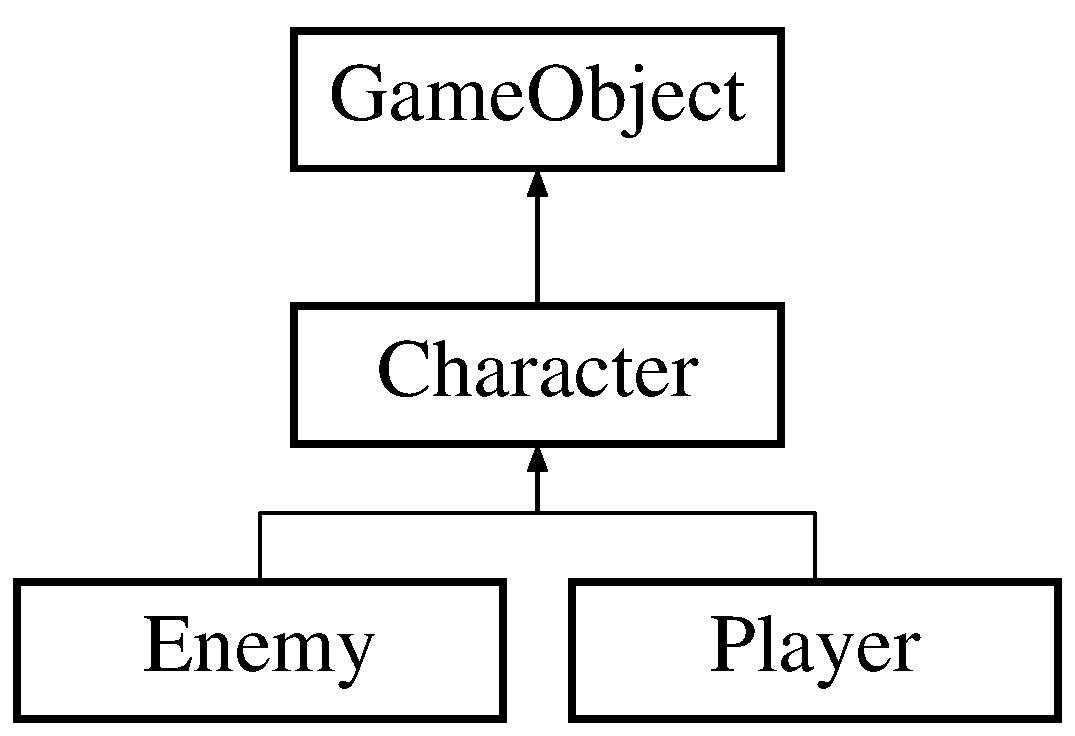
\includegraphics[height=3.000000cm]{class_character}
\end{center}
\end{figure}
\subsection*{Public Member Functions}
\begin{DoxyCompactItemize}
\item 
\mbox{\Hypertarget{class_character_a83f1f8a2eb47e7a891ef14e673703e15}\label{class_character_a83f1f8a2eb47e7a891ef14e673703e15}} 
{\bfseries Character} (const std\+::string, int, int, int)
\item 
\mbox{\Hypertarget{class_character_a5c979ca4dd41c717ff7f6a620c67c0ff}\label{class_character_a5c979ca4dd41c717ff7f6a620c67c0ff}} 
void {\bfseries set\+Lives} (int)
\item 
\mbox{\Hypertarget{class_character_aa49f985b1b05751b2d4b3de74b4acc8c}\label{class_character_aa49f985b1b05751b2d4b3de74b4acc8c}} 
bool {\bfseries is\+Alive} ()
\end{DoxyCompactItemize}


The documentation for this class was generated from the following files\+:\begin{DoxyCompactItemize}
\item 
Character.\+h\item 
Character.\+cpp\end{DoxyCompactItemize}

\hypertarget{class_component_factory}{}\section{Component\+Factory Class Reference}
\label{class_component_factory}\index{Component\+Factory@{Component\+Factory}}


{\ttfamily \#include $<$Component\+Factory.\+h$>$}

\subsection*{Public Member Functions}
\begin{DoxyCompactItemize}
\item 
\mbox{\Hypertarget{class_component_factory_aa6178ddfecc39747ef12f11606735e09}\label{class_component_factory_aa6178ddfecc39747ef12f11606735e09}} 
\mbox{\hyperlink{class_i_storage_manager}{I\+Storage\+Manager}} $\ast$ \mbox{\hyperlink{class_component_factory_aa6178ddfecc39747ef12f11606735e09}{Get\+Storage\+Manager}} ()
\begin{DoxyCompactList}\small\item\em will return a pointer to an object implementing the \mbox{\hyperlink{class_i_storage_manager}{I\+Storage\+Manager}} \end{DoxyCompactList}\item 
\mbox{\Hypertarget{class_component_factory_a84613a5a5f11003abd9d10620ca72b5b}\label{class_component_factory_a84613a5a5f11003abd9d10620ca72b5b}} 
\mbox{\hyperlink{class_i_input_manager}{I\+Input\+Manager}} $\ast$ \mbox{\hyperlink{class_component_factory_a84613a5a5f11003abd9d10620ca72b5b}{Get\+Input\+Manager}} ()
\begin{DoxyCompactList}\small\item\em will return a pointer to an object implementing the \mbox{\hyperlink{class_i_input_manager}{I\+Input\+Manager}} \end{DoxyCompactList}\item 
\mbox{\Hypertarget{class_component_factory_aa8a3b17c86c562cc69f50f283ed3cc28}\label{class_component_factory_aa8a3b17c86c562cc69f50f283ed3cc28}} 
\mbox{\hyperlink{class_i_logic_manager}{I\+Logic\+Manager}} $\ast$ \mbox{\hyperlink{class_component_factory_aa8a3b17c86c562cc69f50f283ed3cc28}{Get\+Logic\+Manager}} ()
\begin{DoxyCompactList}\small\item\em will return a pointer to an object implementing the \mbox{\hyperlink{class_i_logic_manager}{I\+Logic\+Manager}} \end{DoxyCompactList}\item 
\mbox{\Hypertarget{class_component_factory_a19583d4fc53d5942e5c0558a52809086}\label{class_component_factory_a19583d4fc53d5942e5c0558a52809086}} 
\mbox{\hyperlink{class_i_output_manager}{I\+Output\+Manager}} $\ast$ \mbox{\hyperlink{class_component_factory_a19583d4fc53d5942e5c0558a52809086}{Get\+Output\+Manager}} ()
\begin{DoxyCompactList}\small\item\em will return a pointer to an object implementing the \mbox{\hyperlink{class_i_output_manager}{I\+Output\+Manager}} \end{DoxyCompactList}\end{DoxyCompactItemize}


\subsection{Detailed Description}
The purpose of this class is to determine which specific implementations of the components to be used. Example\+: Get\+Storage\+Component might return a \mbox{\hyperlink{class_hard_coded_storage_manager}{Hard\+Coded\+Storage\+Manager}}, or a File\+System\+Storage\+Manager, which both implement the \mbox{\hyperlink{class_i_storage_manager}{I\+Storage\+Manager}} interface. 

The documentation for this class was generated from the following files\+:\begin{DoxyCompactItemize}
\item 
G\+A\+M\+Esource/Component\+Factory.\+h\item 
G\+A\+M\+Esource/Component\+Factory.\+cpp\end{DoxyCompactItemize}

\hypertarget{class_data_toolkit}{}\section{Data\+Toolkit Class Reference}
\label{class_data_toolkit}\index{Data\+Toolkit@{Data\+Toolkit}}
\subsection*{Static Public Member Functions}
\begin{DoxyCompactItemize}
\item 
static std\+::vector$<$ std\+::string $>$ \mbox{\hyperlink{class_data_toolkit_aca86f00861be433066ed7d5f3962c387}{get\+Subs}} (std\+::string s, char delimiter)
\end{DoxyCompactItemize}


\subsection{Member Function Documentation}
\mbox{\Hypertarget{class_data_toolkit_aca86f00861be433066ed7d5f3962c387}\label{class_data_toolkit_aca86f00861be433066ed7d5f3962c387}} 
\index{Data\+Toolkit@{Data\+Toolkit}!get\+Subs@{get\+Subs}}
\index{get\+Subs@{get\+Subs}!Data\+Toolkit@{Data\+Toolkit}}
\subsubsection{\texorpdfstring{get\+Subs()}{getSubs()}}
{\footnotesize\ttfamily std\+::vector$<$ std\+::string $>$ Data\+Toolkit\+::get\+Subs (\begin{DoxyParamCaption}\item[{std\+::string}]{s,  }\item[{char}]{delimiter }\end{DoxyParamCaption})\hspace{0.3cm}{\ttfamily [static]}}

$<$ Creating a vector which stores string values

find the symbol that separates objects (semicolon)

store the data from the beggining of the string to the semicolon (not included)

delete the stored data and the semicolon 

The documentation for this class was generated from the following files\+:\begin{DoxyCompactItemize}
\item 
Data\+Toolkit.\+h\item 
Data\+Toolkit.\+cpp\end{DoxyCompactItemize}

\hypertarget{class_dummy_class}{}\section{Dummy\+Class Class Reference}
\label{class_dummy_class}\index{Dummy\+Class@{Dummy\+Class}}


The documentation for this class was generated from the following files\+:\begin{DoxyCompactItemize}
\item 
Dummy\+Class.\+h\item 
Dummy\+Class.\+cpp\end{DoxyCompactItemize}

\hypertarget{class_enemy}{}\section{Enemy Class Reference}
\label{class_enemy}\index{Enemy@{Enemy}}
Inheritance diagram for Enemy\+:\begin{figure}[H]
\begin{center}
\leavevmode
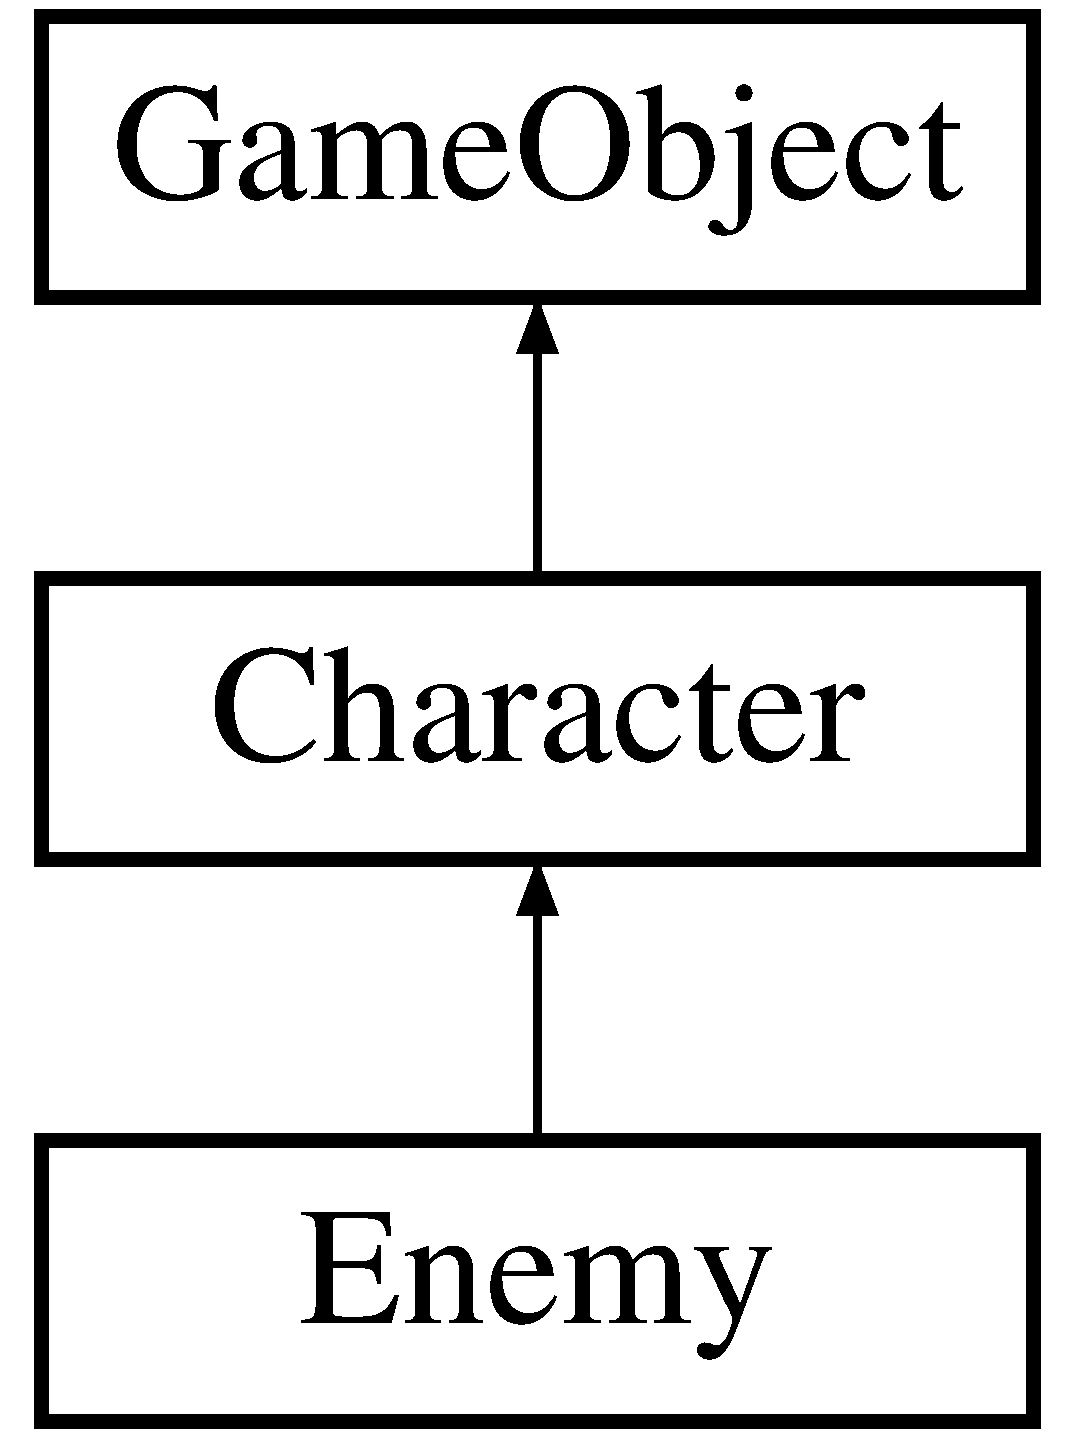
\includegraphics[height=3.000000cm]{class_enemy}
\end{center}
\end{figure}
\subsection*{Public Member Functions}
\begin{DoxyCompactItemize}
\item 
\mbox{\Hypertarget{class_enemy_af847b3e65f5845b7894bc514ca47174b}\label{class_enemy_af847b3e65f5845b7894bc514ca47174b}} 
\mbox{\hyperlink{class_enemy_af847b3e65f5845b7894bc514ca47174b}{Enemy}} (std\+::string, int, int, int, const int)
\begin{DoxyCompactList}\small\item\em constructor \end{DoxyCompactList}\item 
\mbox{\Hypertarget{class_enemy_aafb628c66008e33afdd750e2f492bd98}\label{class_enemy_aafb628c66008e33afdd750e2f492bd98}} 
virtual \mbox{\hyperlink{class_enemy_aafb628c66008e33afdd750e2f492bd98}{$\sim$\+Enemy}} ()=default
\begin{DoxyCompactList}\small\item\em destructor \end{DoxyCompactList}\item 
\mbox{\Hypertarget{class_enemy_abb68708af5f493bee8516d1dce35797e}\label{class_enemy_abb68708af5f493bee8516d1dce35797e}} 
int \mbox{\hyperlink{class_enemy_abb68708af5f493bee8516d1dce35797e}{get\+Damage}} () const
\begin{DoxyCompactList}\small\item\em get the damage \end{DoxyCompactList}\end{DoxyCompactItemize}


The documentation for this class was generated from the following files\+:\begin{DoxyCompactItemize}
\item 
G\+A\+M\+Esource/Enemy.\+h\item 
G\+A\+M\+Esource/Enemy.\+cpp\end{DoxyCompactItemize}

\hypertarget{class_game_level}{}\section{Game\+Level Class Reference}
\label{class_game_level}\index{Game\+Level@{Game\+Level}}


{\ttfamily \#include $<$Game\+Level.\+h$>$}

Inheritance diagram for Game\+Level\+:\begin{figure}[H]
\begin{center}
\leavevmode
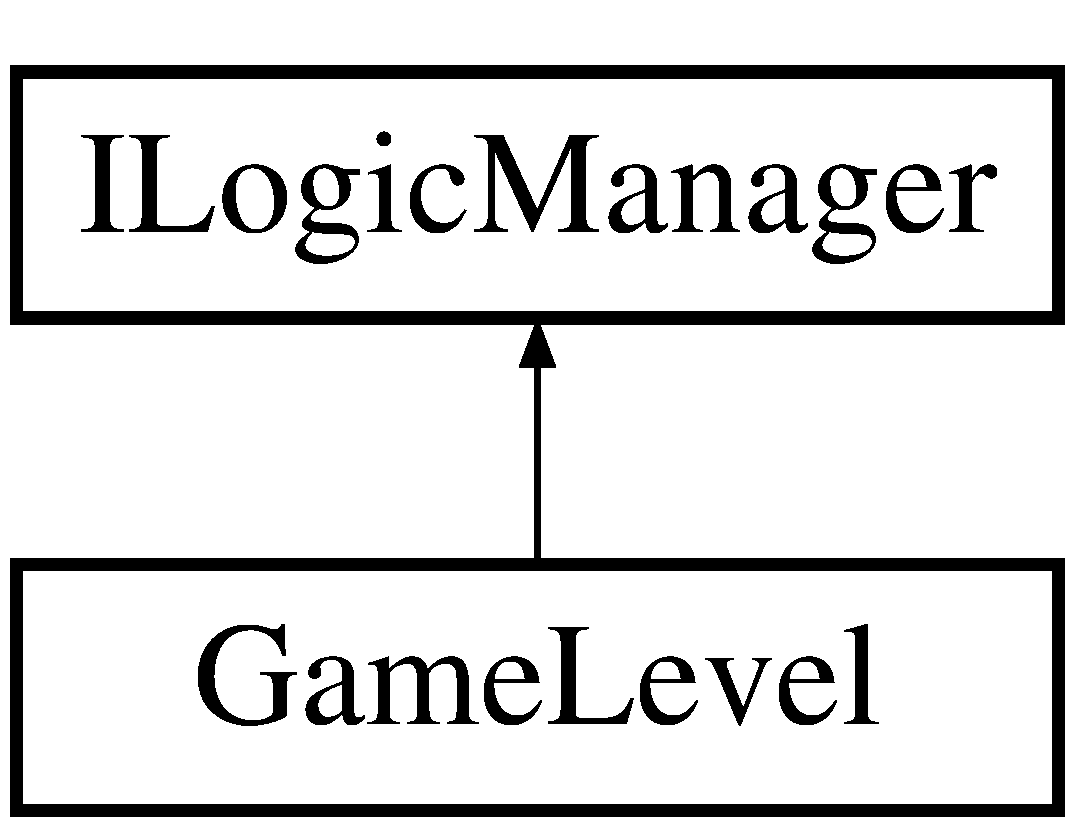
\includegraphics[height=2.000000cm]{class_game_level}
\end{center}
\end{figure}
\subsection*{Public Member Functions}
\begin{DoxyCompactItemize}
\item 
\mbox{\Hypertarget{class_game_level_a5723a38b2b32300d4f071419afacd6f9}\label{class_game_level_a5723a38b2b32300d4f071419afacd6f9}} 
\mbox{\hyperlink{class_game_level_a5723a38b2b32300d4f071419afacd6f9}{Game\+Level}} ()
\begin{DoxyCompactList}\small\item\em constructor \end{DoxyCompactList}\item 
\mbox{\Hypertarget{class_game_level_acbabd989c2876a2326e6b69e33e75fa1}\label{class_game_level_acbabd989c2876a2326e6b69e33e75fa1}} 
void \mbox{\hyperlink{class_game_level_acbabd989c2876a2326e6b69e33e75fa1}{create\+Level}} (\mbox{\hyperlink{class_logic_data}{Logic\+Data}}, bool)
\begin{DoxyCompactList}\small\item\em create all the clases thet form \mbox{\hyperlink{class_game_level}{Game\+Level}} \end{DoxyCompactList}\item 
void \mbox{\hyperlink{class_game_level_a53cd899aa9aeaf3e9579ff32598b0043}{execute\+User\+Command}} (User\+Input\+Type)
\begin{DoxyCompactList}\small\item\em evaluate and perform the user\textquotesingle{}s command \end{DoxyCompactList}\item 
\mbox{\Hypertarget{class_game_level_a89ddaa1423d19132e8d4c97b36f92895}\label{class_game_level_a89ddaa1423d19132e8d4c97b36f92895}} 
std\+::vector$<$ std\+::shared\+\_\+ptr$<$ \mbox{\hyperlink{class_data_update}{Data\+Update}} $>$ $>$ \mbox{\hyperlink{class_game_level_a89ddaa1423d19132e8d4c97b36f92895}{get\+Level\+Updates}} ()
\begin{DoxyCompactList}\small\item\em get objec\textquotesingle{}s data as a vector of strings \end{DoxyCompactList}\item 
\mbox{\Hypertarget{class_game_level_a907f82fea7462dbaf47c396cf65e2e89}\label{class_game_level_a907f82fea7462dbaf47c396cf65e2e89}} 
Game\+State \mbox{\hyperlink{class_game_level_a907f82fea7462dbaf47c396cf65e2e89}{get\+Game\+State}} ()
\begin{DoxyCompactList}\small\item\em check if game is over \end{DoxyCompactList}\end{DoxyCompactItemize}


\subsection{Detailed Description}
Owns different Game\+Oject and level data. Implements the logic part of the game. 

\subsection{Member Function Documentation}
\mbox{\Hypertarget{class_game_level_a53cd899aa9aeaf3e9579ff32598b0043}\label{class_game_level_a53cd899aa9aeaf3e9579ff32598b0043}} 
\index{Game\+Level@{Game\+Level}!execute\+User\+Command@{execute\+User\+Command}}
\index{execute\+User\+Command@{execute\+User\+Command}!Game\+Level@{Game\+Level}}
\subsubsection{\texorpdfstring{execute\+User\+Command()}{executeUserCommand()}}
{\footnotesize\ttfamily void Game\+Level\+::execute\+User\+Command (\begin{DoxyParamCaption}\item[{User\+Input\+Type}]{user\+Input }\end{DoxyParamCaption})\hspace{0.3cm}{\ttfamily [virtual]}}



evaluate and perform the user\textquotesingle{}s command 

execute the input of the data 

Implements \mbox{\hyperlink{class_i_logic_manager_a531478a93285f5cdf6f22294638b27b3}{I\+Logic\+Manager}}.



The documentation for this class was generated from the following files\+:\begin{DoxyCompactItemize}
\item 
G\+A\+M\+Esource/Game\+Level.\+h\item 
G\+A\+M\+Esource/Game\+Level.\+cpp\end{DoxyCompactItemize}

\hypertarget{class_game_manager}{}\section{Game\+Manager Class Reference}
\label{class_game_manager}\index{Game\+Manager@{Game\+Manager}}
\subsection*{Public Member Functions}
\begin{DoxyCompactItemize}
\item 
\mbox{\Hypertarget{class_game_manager_a3af49a72977052275a1217c5018c737f}\label{class_game_manager_a3af49a72977052275a1217c5018c737f}} 
void {\bfseries Start\+Game} ()
\end{DoxyCompactItemize}
\subsection*{Static Public Member Functions}
\begin{DoxyCompactItemize}
\item 
\mbox{\Hypertarget{class_game_manager_acf7198ccac2dde4da381867356136896}\label{class_game_manager_acf7198ccac2dde4da381867356136896}} 
static int {\bfseries Add} (int x, int y)
\end{DoxyCompactItemize}


The documentation for this class was generated from the following files\+:\begin{DoxyCompactItemize}
\item 
Game\+Manager.\+h\item 
Game\+Manager.\+cpp\end{DoxyCompactItemize}

\hypertarget{class_game_object}{}\section{Game\+Object Class Reference}
\label{class_game_object}\index{Game\+Object@{Game\+Object}}


A generic game object that can be moved around. Used in the logic component. Compare \mbox{\hyperlink{class_game_sprite}{Game\+Sprite}}.  




{\ttfamily \#include $<$Game\+Object.\+h$>$}

Inheritance diagram for Game\+Object\+:\begin{figure}[H]
\begin{center}
\leavevmode
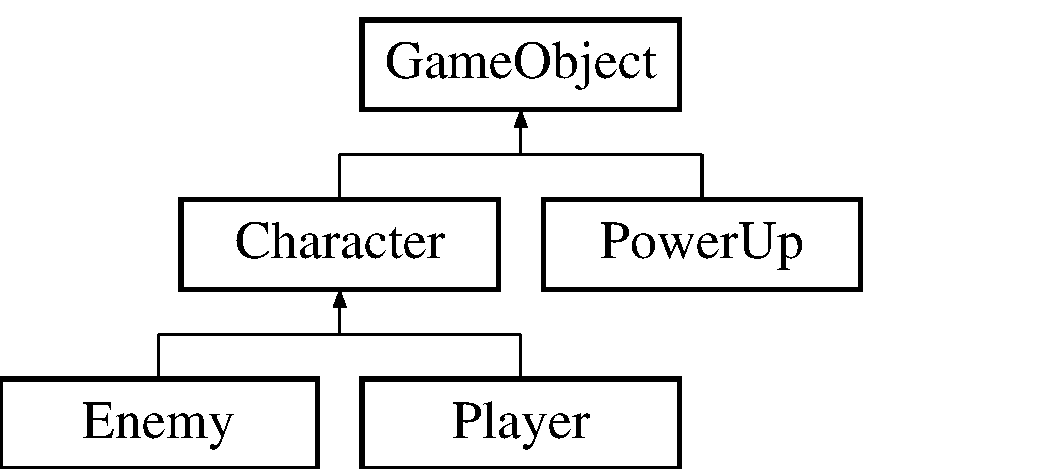
\includegraphics[height=3.000000cm]{class_game_object}
\end{center}
\end{figure}
\subsection*{Public Member Functions}
\begin{DoxyCompactItemize}
\item 
\mbox{\Hypertarget{class_game_object_adf9acb9e2d250f42f322d9b367eb7ff4}\label{class_game_object_adf9acb9e2d250f42f322d9b367eb7ff4}} 
\mbox{\hyperlink{class_game_object_adf9acb9e2d250f42f322d9b367eb7ff4}{Game\+Object}} (std\+::string, int, int)
\begin{DoxyCompactList}\small\item\em constructor \end{DoxyCompactList}\item 
\mbox{\Hypertarget{class_game_object_a67ae2fa6e7916c799700cd659975d8ea}\label{class_game_object_a67ae2fa6e7916c799700cd659975d8ea}} 
virtual \mbox{\hyperlink{class_game_object_a67ae2fa6e7916c799700cd659975d8ea}{$\sim$\+Game\+Object}} ()=default
\begin{DoxyCompactList}\small\item\em vitual destructor \end{DoxyCompactList}\item 
\mbox{\Hypertarget{class_game_object_a54cb68b217bc51148649d10dc4f9bcbf}\label{class_game_object_a54cb68b217bc51148649d10dc4f9bcbf}} 
std\+::string \mbox{\hyperlink{class_game_object_a54cb68b217bc51148649d10dc4f9bcbf}{get\+ID}} ()
\begin{DoxyCompactList}\small\item\em get object ID \end{DoxyCompactList}\item 
\mbox{\Hypertarget{class_game_object_af1468b4adeb7ac7218b9bfd508a04bd6}\label{class_game_object_af1468b4adeb7ac7218b9bfd508a04bd6}} 
void \mbox{\hyperlink{class_game_object_af1468b4adeb7ac7218b9bfd508a04bd6}{set\+X\+Position}} (int)
\begin{DoxyCompactList}\small\item\em set x-\/position \end{DoxyCompactList}\item 
\mbox{\Hypertarget{class_game_object_ab5e682e5f30212535f21b00f7ac5aa7d}\label{class_game_object_ab5e682e5f30212535f21b00f7ac5aa7d}} 
int \mbox{\hyperlink{class_game_object_ab5e682e5f30212535f21b00f7ac5aa7d}{get\+X\+Position}} ()
\begin{DoxyCompactList}\small\item\em get x-\/position \end{DoxyCompactList}\item 
\mbox{\Hypertarget{class_game_object_a09913a2ffb23b697a0d79bf1145c0f01}\label{class_game_object_a09913a2ffb23b697a0d79bf1145c0f01}} 
void \mbox{\hyperlink{class_game_object_a09913a2ffb23b697a0d79bf1145c0f01}{set\+Y\+Position}} (int)
\begin{DoxyCompactList}\small\item\em set y-\/position \end{DoxyCompactList}\item 
\mbox{\Hypertarget{class_game_object_a2c986fbc8dc62a1c187466a4ab48bebd}\label{class_game_object_a2c986fbc8dc62a1c187466a4ab48bebd}} 
int \mbox{\hyperlink{class_game_object_a2c986fbc8dc62a1c187466a4ab48bebd}{get\+Y\+Position}} ()
\begin{DoxyCompactList}\small\item\em get y-\/position \end{DoxyCompactList}\item 
\mbox{\Hypertarget{class_game_object_af9bc07709ad106c507cccdef63d86254}\label{class_game_object_af9bc07709ad106c507cccdef63d86254}} 
virtual std\+::string \mbox{\hyperlink{class_game_object_af9bc07709ad106c507cccdef63d86254}{data\+To\+String}} ()
\begin{DoxyCompactList}\small\item\em save the data in a string \end{DoxyCompactList}\end{DoxyCompactItemize}


\subsection{Detailed Description}
A generic game object that can be moved around. Used in the logic component. Compare \mbox{\hyperlink{class_game_sprite}{Game\+Sprite}}. 

The documentation for this class was generated from the following files\+:\begin{DoxyCompactItemize}
\item 
G\+A\+M\+Esource/logic/Game\+Object.\+h\item 
G\+A\+M\+Esource/logic/Game\+Object.\+cpp\end{DoxyCompactItemize}

\hypertarget{class_game_sprite}{}\section{Game\+Sprite Class Reference}
\label{class_game_sprite}\index{Game\+Sprite@{Game\+Sprite}}


A generic sprite/tile that can be moved around. Compare \mbox{\hyperlink{class_game_object}{Game\+Object}}.  




{\ttfamily \#include $<$Game\+Sprite.\+h$>$}

Inheritance diagram for Game\+Sprite\+:\begin{figure}[H]
\begin{center}
\leavevmode
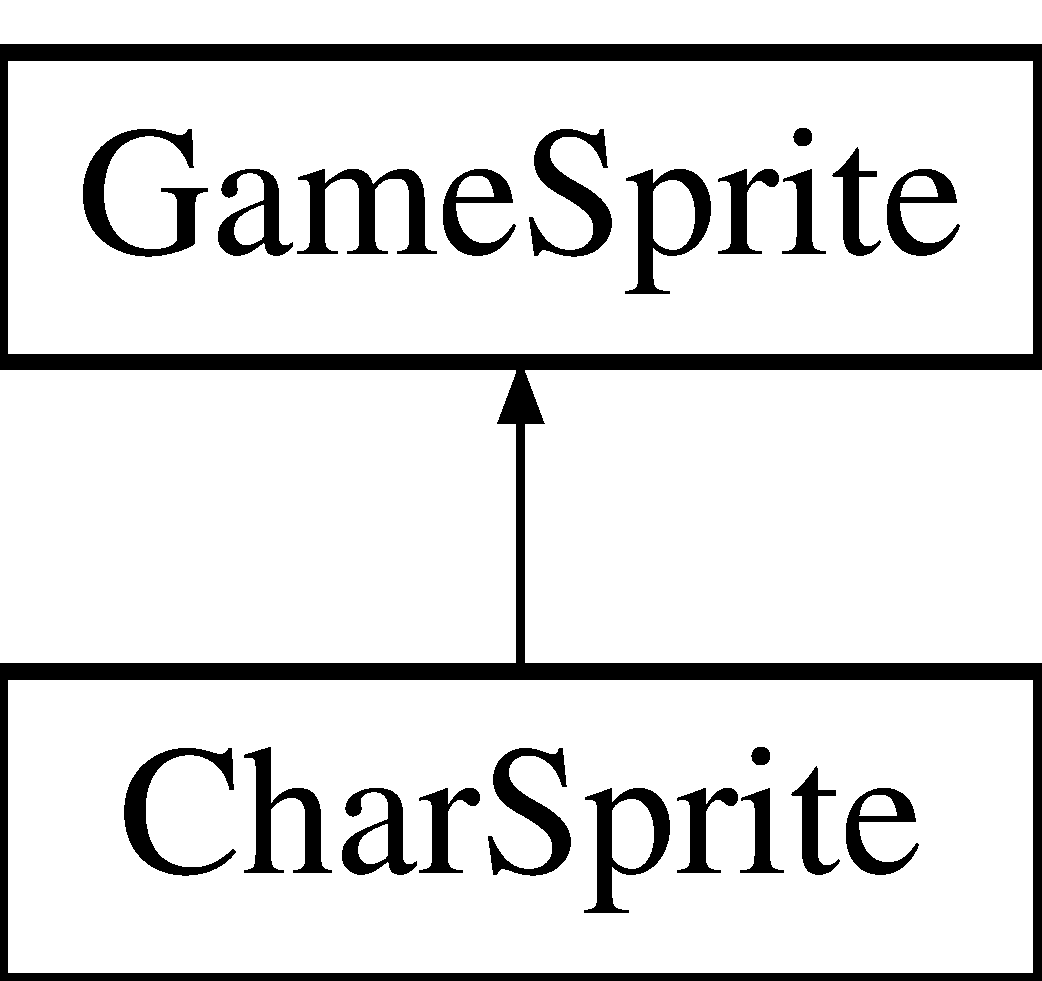
\includegraphics[height=2.000000cm]{class_game_sprite}
\end{center}
\end{figure}
\subsection*{Public Member Functions}
\begin{DoxyCompactItemize}
\item 
\mbox{\Hypertarget{class_game_sprite_aa5e7e9276033b85ebe41123bf9e203f4}\label{class_game_sprite_aa5e7e9276033b85ebe41123bf9e203f4}} 
{\bfseries Game\+Sprite} (int, int, \mbox{\hyperlink{namespace_sprite_attributes_afb5447c311bc29f0ce8ddfd025c6e998}{Sprite\+Attributes\+::\+Art\+Type}}, \mbox{\hyperlink{namespace_sprite_attributes_a3ece96d6288b14d53d84e2138392395c}{Sprite\+Attributes\+::\+Description}}, \mbox{\hyperlink{namespace_sprite_attributes_a254503d1929a87fa82146c9b7d19c2df}{Sprite\+Attributes\+::\+Tile\+Type}})
\item 
\mbox{\Hypertarget{class_game_sprite_a58f1b3fce8064be9921bd37869e9b117}\label{class_game_sprite_a58f1b3fce8064be9921bd37869e9b117}} 
void \mbox{\hyperlink{class_game_sprite_a58f1b3fce8064be9921bd37869e9b117}{set\+Type}} (\mbox{\hyperlink{namespace_sprite_attributes_afb5447c311bc29f0ce8ddfd025c6e998}{Sprite\+Attributes\+::\+Art\+Type}})
\begin{DoxyCompactList}\small\item\em set sprite artwork \end{DoxyCompactList}\item 
\mbox{\Hypertarget{class_game_sprite_a7125087aa8a0c333a7aa6835ecf8c6c8}\label{class_game_sprite_a7125087aa8a0c333a7aa6835ecf8c6c8}} 
\mbox{\hyperlink{namespace_sprite_attributes_afb5447c311bc29f0ce8ddfd025c6e998}{Sprite\+Attributes\+::\+Art\+Type}} \mbox{\hyperlink{class_game_sprite_a7125087aa8a0c333a7aa6835ecf8c6c8}{get\+Art}} ()
\begin{DoxyCompactList}\small\item\em get sprite artwork \end{DoxyCompactList}\item 
\mbox{\Hypertarget{class_game_sprite_a28d3d766c1f6cacc84445fdfe5b6e25e}\label{class_game_sprite_a28d3d766c1f6cacc84445fdfe5b6e25e}} 
void \mbox{\hyperlink{class_game_sprite_a28d3d766c1f6cacc84445fdfe5b6e25e}{set\+Description}} (\mbox{\hyperlink{namespace_sprite_attributes_a3ece96d6288b14d53d84e2138392395c}{Sprite\+Attributes\+::\+Description}})
\begin{DoxyCompactList}\small\item\em set sprite artwork description \end{DoxyCompactList}\item 
\mbox{\Hypertarget{class_game_sprite_a2ca8b811d79fbceae18e02c934e3e85b}\label{class_game_sprite_a2ca8b811d79fbceae18e02c934e3e85b}} 
\mbox{\hyperlink{namespace_sprite_attributes_a3ece96d6288b14d53d84e2138392395c}{Sprite\+Attributes\+::\+Description}} \mbox{\hyperlink{class_game_sprite_a2ca8b811d79fbceae18e02c934e3e85b}{get\+Description}} ()
\begin{DoxyCompactList}\small\item\em get sprite artwork description \end{DoxyCompactList}\item 
\mbox{\Hypertarget{class_game_sprite_a1cb6989acf2cc9666be1bc940b31d7c7}\label{class_game_sprite_a1cb6989acf2cc9666be1bc940b31d7c7}} 
virtual void \mbox{\hyperlink{class_game_sprite_a1cb6989acf2cc9666be1bc940b31d7c7}{move\+Sprite}} (int, int)
\begin{DoxyCompactList}\small\item\em move sprite to a x and y position, no orientation taken into account \end{DoxyCompactList}\item 
\mbox{\Hypertarget{class_game_sprite_a35eac21d4f5d7e23d1bdd22b1e6a8517}\label{class_game_sprite_a35eac21d4f5d7e23d1bdd22b1e6a8517}} 
virtual void \mbox{\hyperlink{class_game_sprite_a35eac21d4f5d7e23d1bdd22b1e6a8517}{move\+Sprite}} (int)
\begin{DoxyCompactList}\small\item\em Define virtual functions for use with more complex \mbox{\hyperlink{class_game_sprite}{Game\+Sprite}} child classes. \end{DoxyCompactList}\item 
\mbox{\Hypertarget{class_game_sprite_acf5168b8fa90814756fa660aabf6da70}\label{class_game_sprite_acf5168b8fa90814756fa660aabf6da70}} 
void \mbox{\hyperlink{class_game_sprite_acf5168b8fa90814756fa660aabf6da70}{move\+Sprite}} (User\+Input\+Type, int)
\begin{DoxyCompactList}\small\item\em For test purposes only, as this is not connected to the logic. \end{DoxyCompactList}\item 
\mbox{\Hypertarget{class_game_sprite_acb65331428a0ae05f1ef6f521d51e4e7}\label{class_game_sprite_acb65331428a0ae05f1ef6f521d51e4e7}} 
virtual void \mbox{\hyperlink{class_game_sprite_acb65331428a0ae05f1ef6f521d51e4e7}{set\+Orientation}} (Character\+Orientation)
\begin{DoxyCompactList}\small\item\em Define virtual functions for use with more complex \mbox{\hyperlink{class_game_sprite}{Game\+Sprite}} child classes. \end{DoxyCompactList}\item 
\mbox{\Hypertarget{class_game_sprite_aecf8f0273b4e847aa532f8980fb78997}\label{class_game_sprite_aecf8f0273b4e847aa532f8980fb78997}} 
virtual Character\+Orientation \mbox{\hyperlink{class_game_sprite_aecf8f0273b4e847aa532f8980fb78997}{get\+Orientation}} ()
\begin{DoxyCompactList}\small\item\em Return Character\+Orientation\+::\+None. \end{DoxyCompactList}\item 
\mbox{\Hypertarget{class_game_sprite_adcd973ba50bc01f1a5a8e81d7e468be3}\label{class_game_sprite_adcd973ba50bc01f1a5a8e81d7e468be3}} 
void \mbox{\hyperlink{class_game_sprite_adcd973ba50bc01f1a5a8e81d7e468be3}{set\+X\+Position}} (int)
\begin{DoxyCompactList}\small\item\em set X-\/\+Position \end{DoxyCompactList}\item 
\mbox{\Hypertarget{class_game_sprite_adf371cf5b8636f7cfd8cb998460f7053}\label{class_game_sprite_adf371cf5b8636f7cfd8cb998460f7053}} 
int \mbox{\hyperlink{class_game_sprite_adf371cf5b8636f7cfd8cb998460f7053}{get\+X\+Position}} ()
\begin{DoxyCompactList}\small\item\em get X-\/\+Position \end{DoxyCompactList}\item 
\mbox{\Hypertarget{class_game_sprite_a31f481d89973565bb2d0d55d0600c266}\label{class_game_sprite_a31f481d89973565bb2d0d55d0600c266}} 
void \mbox{\hyperlink{class_game_sprite_a31f481d89973565bb2d0d55d0600c266}{set\+Y\+Position}} (int)
\begin{DoxyCompactList}\small\item\em get Y-\/\+Position \end{DoxyCompactList}\item 
\mbox{\Hypertarget{class_game_sprite_aea645d5397fc4cdbd386e3133e33a802}\label{class_game_sprite_aea645d5397fc4cdbd386e3133e33a802}} 
int \mbox{\hyperlink{class_game_sprite_aea645d5397fc4cdbd386e3133e33a802}{get\+Y\+Position}} ()
\begin{DoxyCompactList}\small\item\em get Y-\/\+Position \end{DoxyCompactList}\end{DoxyCompactItemize}
\subsection*{Public Attributes}
\begin{DoxyCompactItemize}
\item 
\mbox{\Hypertarget{class_game_sprite_a8cba19cb70bb128532903b320a0065c9}\label{class_game_sprite_a8cba19cb70bb128532903b320a0065c9}} 
\mbox{\hyperlink{namespace_sprite_attributes_a254503d1929a87fa82146c9b7d19c2df}{Sprite\+Attributes\+::\+Tile\+Type}} \mbox{\hyperlink{class_game_sprite_a8cba19cb70bb128532903b320a0065c9}{tm}}
\begin{DoxyCompactList}\small\item\em define which tile\+Manager to use with this sprite \end{DoxyCompactList}\end{DoxyCompactItemize}


\subsection{Detailed Description}
A generic sprite/tile that can be moved around. Compare \mbox{\hyperlink{class_game_object}{Game\+Object}}. 

The documentation for this class was generated from the following files\+:\begin{DoxyCompactItemize}
\item 
G\+A\+M\+Esource/output/Game\+Sprite.\+h\item 
G\+A\+M\+Esource/output/Game\+Sprite.\+cpp\end{DoxyCompactItemize}

\hypertarget{class_graphic_interface}{}\section{Graphic\+Interface Class Reference}
\label{class_graphic_interface}\index{Graphic\+Interface@{Graphic\+Interface}}
Inheritance diagram for Graphic\+Interface\+:\begin{figure}[H]
\begin{center}
\leavevmode
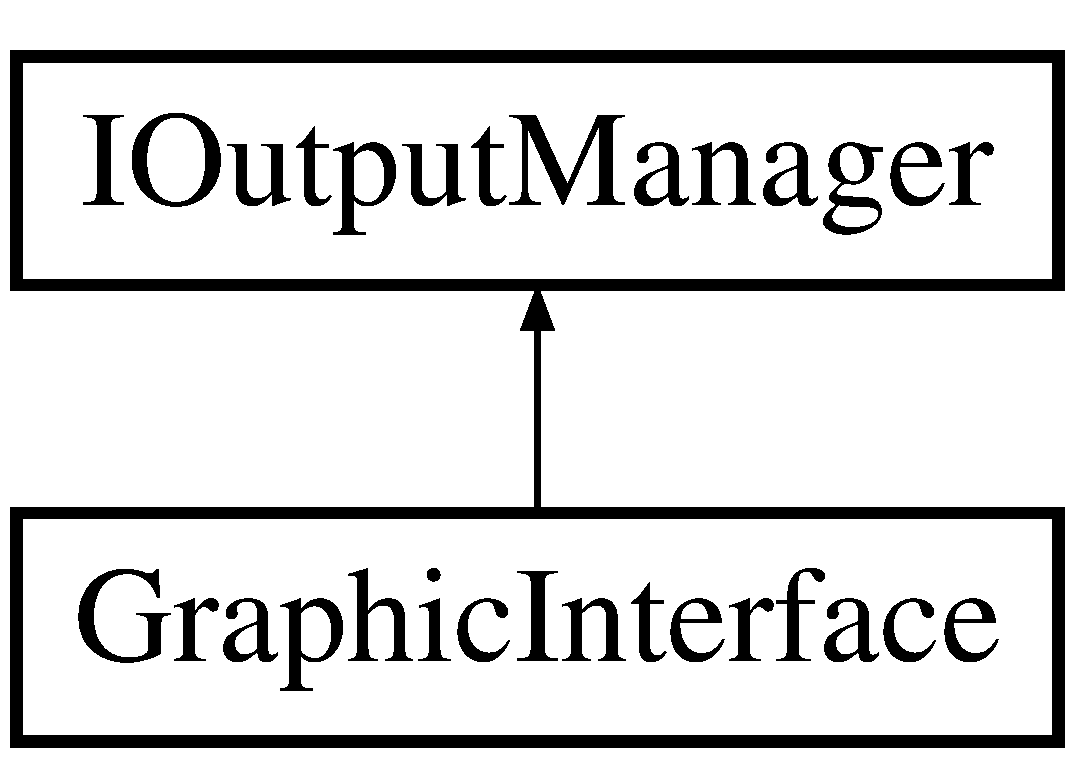
\includegraphics[height=2.000000cm]{class_graphic_interface}
\end{center}
\end{figure}
\subsection*{Public Member Functions}
\begin{DoxyCompactItemize}
\item 
\mbox{\hyperlink{class_graphic_interface_accff331d036826a9c43e7bcd39165dc2}{Graphic\+Interface}} ()
\item 
\mbox{\Hypertarget{class_graphic_interface_ad36aed285f05abff15f0991810ea2bde}\label{class_graphic_interface_ad36aed285f05abff15f0991810ea2bde}} 
\mbox{\hyperlink{class_graphic_interface_ad36aed285f05abff15f0991810ea2bde}{Graphic\+Interface}} (const \mbox{\hyperlink{class_graphic_interface}{Graphic\+Interface}} \&)=delete
\begin{DoxyCompactList}\small\item\em UI objects should not be copied or moved. \end{DoxyCompactList}\item 
\mbox{\Hypertarget{class_graphic_interface_aa89a56ec49a83a0f6ae3de05c86d6e80}\label{class_graphic_interface_aa89a56ec49a83a0f6ae3de05c86d6e80}} 
{\bfseries Graphic\+Interface} (const \mbox{\hyperlink{class_graphic_interface}{Graphic\+Interface}} \&\&)=delete
\item 
\mbox{\Hypertarget{class_graphic_interface_ac7bd13606ffcf7c14e35990c3ad4d868}\label{class_graphic_interface_ac7bd13606ffcf7c14e35990c3ad4d868}} 
\mbox{\hyperlink{class_graphic_interface}{Graphic\+Interface}} \& {\bfseries operator=} (const \mbox{\hyperlink{class_graphic_interface}{Graphic\+Interface}} \&)=delete
\item 
\mbox{\hyperlink{class_graphic_interface_a48f212964040a5baf30035420305c1f9}{$\sim$\+Graphic\+Interface}} ()
\item 
void \mbox{\hyperlink{class_graphic_interface_a4237627c03422b22653a3a462bd1daa2}{load\+Level}} (\mbox{\hyperlink{class_output_data}{Output\+Data}})
\item 
void \mbox{\hyperlink{class_graphic_interface_a250275a6b20097a3c3435a9af4d1cd75}{update}} (std\+::vector$<$ std\+::string $>$ data)
\item 
void \mbox{\hyperlink{class_graphic_interface_abb3581948def6522f616e9f3ce1c40ac}{update}} (User\+Input\+Type)
\item 
\mbox{\Hypertarget{class_graphic_interface_adc91101675b7727393c747a06db7e4e2}\label{class_graphic_interface_adc91101675b7727393c747a06db7e4e2}} 
void \mbox{\hyperlink{class_graphic_interface_adc91101675b7727393c747a06db7e4e2}{show\+Game\+Over\+Screen}} ()
\begin{DoxyCompactList}\small\item\em Displays the Game Over screen. \end{DoxyCompactList}\item 
void \mbox{\hyperlink{class_graphic_interface_a2a52c6fef543c4f130f62ee4552648f9}{move\+Sprite}} (\mbox{\hyperlink{class_game_sprite}{Game\+Sprite}} $\ast$, int, int)
\item 
void \mbox{\hyperlink{class_graphic_interface_a8062b59b90fa4075903ddc122f2ba8ed}{move\+Sprite}} (User\+Input\+Type, std\+::string)
\end{DoxyCompactItemize}


\subsection{Constructor \& Destructor Documentation}
\mbox{\Hypertarget{class_graphic_interface_accff331d036826a9c43e7bcd39165dc2}\label{class_graphic_interface_accff331d036826a9c43e7bcd39165dc2}} 
\index{Graphic\+Interface@{Graphic\+Interface}!Graphic\+Interface@{Graphic\+Interface}}
\index{Graphic\+Interface@{Graphic\+Interface}!Graphic\+Interface@{Graphic\+Interface}}
\subsubsection{\texorpdfstring{Graphic\+Interface()}{GraphicInterface()}}
{\footnotesize\ttfamily Graphic\+Interface\+::\+Graphic\+Interface (\begin{DoxyParamCaption}{ }\end{DoxyParamCaption})}

Constructor Note\+: all initialisation is done in Graphic\+Interface\+::loadlevel() \mbox{\Hypertarget{class_graphic_interface_a48f212964040a5baf30035420305c1f9}\label{class_graphic_interface_a48f212964040a5baf30035420305c1f9}} 
\index{Graphic\+Interface@{Graphic\+Interface}!````~Graphic\+Interface@{$\sim$\+Graphic\+Interface}}
\index{````~Graphic\+Interface@{$\sim$\+Graphic\+Interface}!Graphic\+Interface@{Graphic\+Interface}}
\subsubsection{\texorpdfstring{$\sim$\+Graphic\+Interface()}{~GraphicInterface()}}
{\footnotesize\ttfamily Graphic\+Interface\+::$\sim$\+Graphic\+Interface (\begin{DoxyParamCaption}{ }\end{DoxyParamCaption})}

Destructor Fully de-\/initializes the UI, including closing the main window. 

\subsection{Member Function Documentation}
\mbox{\Hypertarget{class_graphic_interface_a4237627c03422b22653a3a462bd1daa2}\label{class_graphic_interface_a4237627c03422b22653a3a462bd1daa2}} 
\index{Graphic\+Interface@{Graphic\+Interface}!load\+Level@{load\+Level}}
\index{load\+Level@{load\+Level}!Graphic\+Interface@{Graphic\+Interface}}
\subsubsection{\texorpdfstring{load\+Level()}{loadLevel()}}
{\footnotesize\ttfamily void Graphic\+Interface\+::load\+Level (\begin{DoxyParamCaption}\item[{\mbox{\hyperlink{class_output_data}{Output\+Data}}}]{input\+String }\end{DoxyParamCaption})\hspace{0.3cm}{\ttfamily [virtual]}}

Initialize the UI fully. Loads data Creates a main (S\+DL) window for rendering, and loads the sprites from a bitmap on disk. Public because called by Game Manager 

Implements \mbox{\hyperlink{class_i_output_manager_a50a935d76cf10427b0977406a2338146}{I\+Output\+Manager}}.

\mbox{\Hypertarget{class_graphic_interface_a2a52c6fef543c4f130f62ee4552648f9}\label{class_graphic_interface_a2a52c6fef543c4f130f62ee4552648f9}} 
\index{Graphic\+Interface@{Graphic\+Interface}!move\+Sprite@{move\+Sprite}}
\index{move\+Sprite@{move\+Sprite}!Graphic\+Interface@{Graphic\+Interface}}
\subsubsection{\texorpdfstring{move\+Sprite()}{moveSprite()}\hspace{0.1cm}{\footnotesize\ttfamily [1/2]}}
{\footnotesize\ttfamily void Graphic\+Interface\+::move\+Sprite (\begin{DoxyParamCaption}\item[{\mbox{\hyperlink{class_game_sprite}{Game\+Sprite}} $\ast$}]{element,  }\item[{int}]{x,  }\item[{int}]{y }\end{DoxyParamCaption})}

Move a sprite to a position Data is given by the logic manager \mbox{\Hypertarget{class_graphic_interface_a8062b59b90fa4075903ddc122f2ba8ed}\label{class_graphic_interface_a8062b59b90fa4075903ddc122f2ba8ed}} 
\index{Graphic\+Interface@{Graphic\+Interface}!move\+Sprite@{move\+Sprite}}
\index{move\+Sprite@{move\+Sprite}!Graphic\+Interface@{Graphic\+Interface}}
\subsubsection{\texorpdfstring{move\+Sprite()}{moveSprite()}\hspace{0.1cm}{\footnotesize\ttfamily [2/2]}}
{\footnotesize\ttfamily void Graphic\+Interface\+::move\+Sprite (\begin{DoxyParamCaption}\item[{User\+Input\+Type}]{command,  }\item[{std\+::string}]{ID }\end{DoxyParamCaption})}

Move a sprite on the screen using user input. For test purposes only, as this is not connected to the logic \mbox{\Hypertarget{class_graphic_interface_a250275a6b20097a3c3435a9af4d1cd75}\label{class_graphic_interface_a250275a6b20097a3c3435a9af4d1cd75}} 
\index{Graphic\+Interface@{Graphic\+Interface}!update@{update}}
\index{update@{update}!Graphic\+Interface@{Graphic\+Interface}}
\subsubsection{\texorpdfstring{update()}{update()}\hspace{0.1cm}{\footnotesize\ttfamily [1/2]}}
{\footnotesize\ttfamily void Graphic\+Interface\+::update (\begin{DoxyParamCaption}\item[{std\+::vector$<$ std\+::string $>$}]{data }\end{DoxyParamCaption})\hspace{0.3cm}{\ttfamily [virtual]}}

Update the screen
\begin{DoxyItemize}
\item Draw the background
\item Draw the score
\item Draw the remaining lives
\item Draw the objects (last) 
\end{DoxyItemize}

Implements \mbox{\hyperlink{class_i_output_manager_aaebb6c7029ac00c7ce293272a5e854e3}{I\+Output\+Manager}}.

\mbox{\Hypertarget{class_graphic_interface_abb3581948def6522f616e9f3ce1c40ac}\label{class_graphic_interface_abb3581948def6522f616e9f3ce1c40ac}} 
\index{Graphic\+Interface@{Graphic\+Interface}!update@{update}}
\index{update@{update}!Graphic\+Interface@{Graphic\+Interface}}
\subsubsection{\texorpdfstring{update()}{update()}\hspace{0.1cm}{\footnotesize\ttfamily [2/2]}}
{\footnotesize\ttfamily void Graphic\+Interface\+::update (\begin{DoxyParamCaption}\item[{User\+Input\+Type}]{user\+Input }\end{DoxyParamCaption})\hspace{0.3cm}{\ttfamily [virtual]}}

A test update that takes in user inputs directly, so that the logic component can be completely bypassed This is useful for testing animations 

Implements \mbox{\hyperlink{class_i_output_manager_aef1aaf499f3eee5927cb2833af39ce43}{I\+Output\+Manager}}.



The documentation for this class was generated from the following files\+:\begin{DoxyCompactItemize}
\item 
C\+:/\+Users/\+User/source/repos/\+G\+A\+M\+E/\+G\+A\+M\+Esource/Graphic\+Interface.\+h\item 
C\+:/\+Users/\+User/source/repos/\+G\+A\+M\+E/\+G\+A\+M\+Esource/Graphic\+Interface.\+cpp\end{DoxyCompactItemize}

\hypertarget{class_hard_coded_storage_manager}{}\section{Hard\+Coded\+Storage\+Manager Class Reference}
\label{class_hard_coded_storage_manager}\index{Hard\+Coded\+Storage\+Manager@{Hard\+Coded\+Storage\+Manager}}
Inheritance diagram for Hard\+Coded\+Storage\+Manager\+:\begin{figure}[H]
\begin{center}
\leavevmode
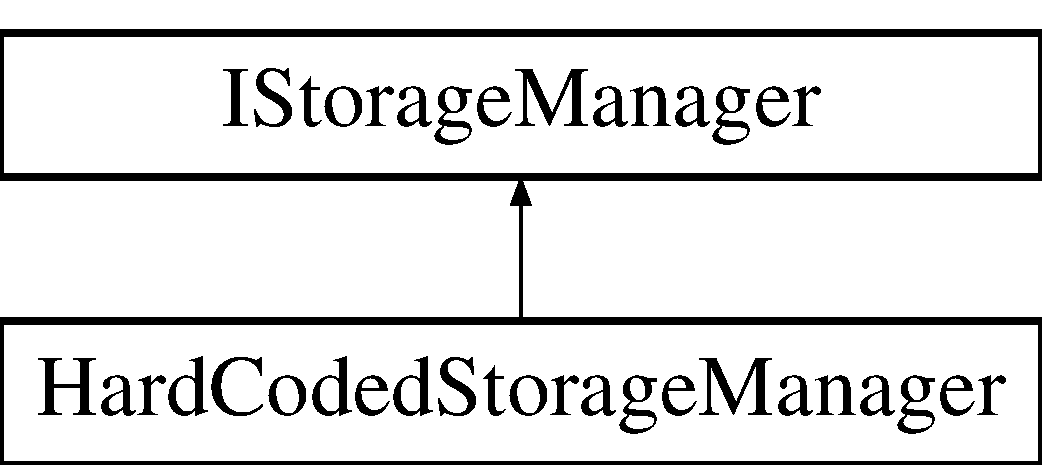
\includegraphics[height=2.000000cm]{class_hard_coded_storage_manager}
\end{center}
\end{figure}
\subsection*{Public Member Functions}
\begin{DoxyCompactItemize}
\item 
\mbox{\Hypertarget{class_hard_coded_storage_manager_a63cb0028398459428f52c88640daf274}\label{class_hard_coded_storage_manager_a63cb0028398459428f52c88640daf274}} 
\mbox{\hyperlink{class_storage_data}{Storage\+Data}} $\ast$ {\bfseries load\+Default\+Level} ()
\end{DoxyCompactItemize}


The documentation for this class was generated from the following files\+:\begin{DoxyCompactItemize}
\item 
Hard\+Coded\+Storage\+Manager.\+h\item 
Hard\+Coded\+Storage\+Manager.\+cpp\end{DoxyCompactItemize}

\hypertarget{class_i_input_manager}{}\section{I\+Input\+Manager Class Reference}
\label{class_i_input_manager}\index{I\+Input\+Manager@{I\+Input\+Manager}}


{\ttfamily \#include $<$I\+Input\+Manager.\+h$>$}

Inheritance diagram for I\+Input\+Manager\+:\begin{figure}[H]
\begin{center}
\leavevmode
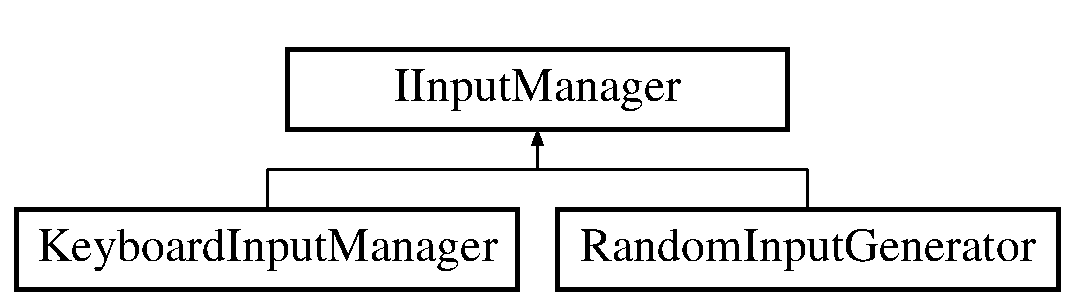
\includegraphics[height=2.000000cm]{class_i_input_manager}
\end{center}
\end{figure}
\subsection*{Public Member Functions}
\begin{DoxyCompactItemize}
\item 
\mbox{\Hypertarget{class_i_input_manager_aa81a10b1ddf305df10c4aebe6930ac86}\label{class_i_input_manager_aa81a10b1ddf305df10c4aebe6930ac86}} 
virtual \mbox{\hyperlink{class_i_input_manager_aa81a10b1ddf305df10c4aebe6930ac86}{$\sim$\+I\+Input\+Manager}} ()=0
\begin{DoxyCompactList}\small\item\em virtual destructor to be implemented in the class implementing the interface \end{DoxyCompactList}\item 
\mbox{\Hypertarget{class_i_input_manager_afa367fc9694f45150aeb59039dcd4421}\label{class_i_input_manager_afa367fc9694f45150aeb59039dcd4421}} 
virtual User\+Input\+Type \mbox{\hyperlink{class_i_input_manager_afa367fc9694f45150aeb59039dcd4421}{get\+Input}} ()=0
\begin{DoxyCompactList}\small\item\em Provides a single input from whichever source mapped as User\+Input\+Type. \end{DoxyCompactList}\end{DoxyCompactItemize}


\subsection{Detailed Description}
Interface to be implemented by a class acting as the manager of the Input Component 

The documentation for this class was generated from the following files\+:\begin{DoxyCompactItemize}
\item 
G\+A\+M\+Esource/I\+Input\+Manager.\+h\item 
G\+A\+M\+Esource/I\+Input\+Manager.\+cpp\end{DoxyCompactItemize}

\hypertarget{class_i_logic_manager}{}\section{I\+Logic\+Manager Class Reference}
\label{class_i_logic_manager}\index{I\+Logic\+Manager@{I\+Logic\+Manager}}


Interface to be implemented by a class acting as the manager of the Logic Component.  




{\ttfamily \#include $<$I\+Logic\+Manager.\+h$>$}

Inheritance diagram for I\+Logic\+Manager\+:\begin{figure}[H]
\begin{center}
\leavevmode
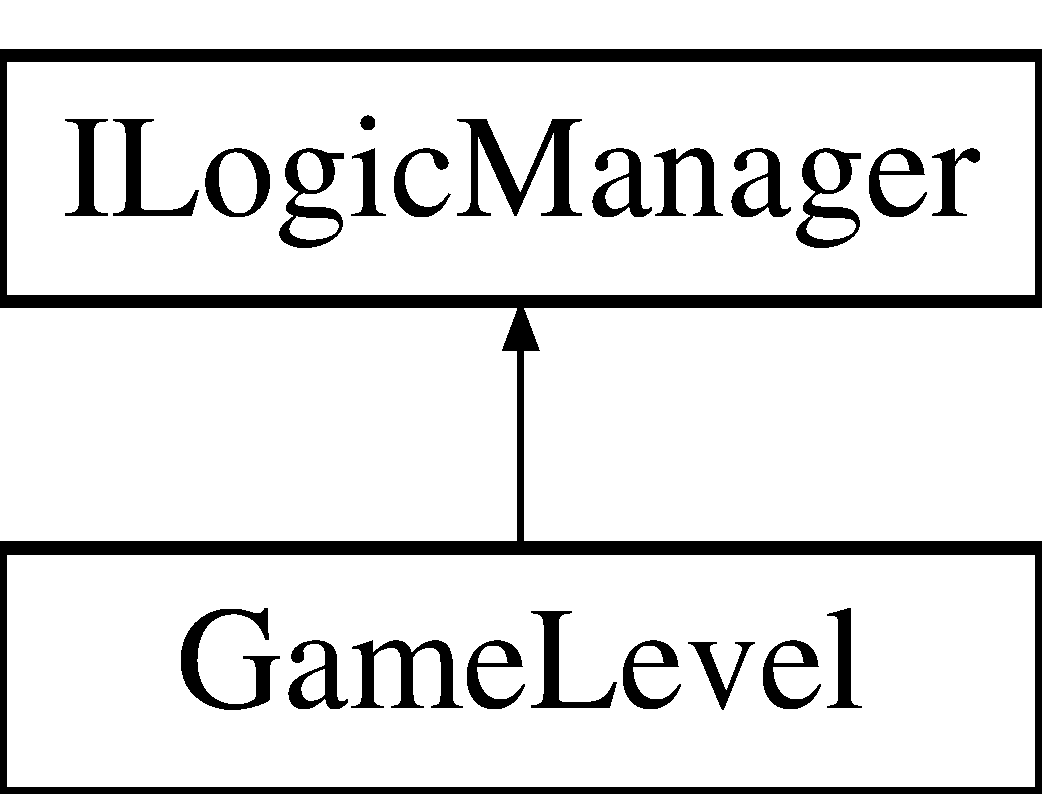
\includegraphics[height=2.000000cm]{class_i_logic_manager}
\end{center}
\end{figure}
\subsection*{Public Member Functions}
\begin{DoxyCompactItemize}
\item 
\mbox{\Hypertarget{class_i_logic_manager_af522c957cdce66d34eb8264212b413ed}\label{class_i_logic_manager_af522c957cdce66d34eb8264212b413ed}} 
virtual \mbox{\hyperlink{class_i_logic_manager_af522c957cdce66d34eb8264212b413ed}{$\sim$\+I\+Logic\+Manager}} ()=0
\begin{DoxyCompactList}\small\item\em virtual destructor to be implemented in the class implementing the interface \end{DoxyCompactList}\item 
\mbox{\Hypertarget{class_i_logic_manager_a9d09e24fdfa312e3a908c0110e305ed5}\label{class_i_logic_manager_a9d09e24fdfa312e3a908c0110e305ed5}} 
virtual void \mbox{\hyperlink{class_i_logic_manager_a9d09e24fdfa312e3a908c0110e305ed5}{create\+Level}} (\mbox{\hyperlink{class_logic_data}{Logic\+Data}} level, bool)=0
\begin{DoxyCompactList}\small\item\em create game level \end{DoxyCompactList}\item 
\mbox{\Hypertarget{class_i_logic_manager_a531478a93285f5cdf6f22294638b27b3}\label{class_i_logic_manager_a531478a93285f5cdf6f22294638b27b3}} 
virtual void \mbox{\hyperlink{class_i_logic_manager_a531478a93285f5cdf6f22294638b27b3}{execute\+User\+Command}} (User\+Input\+Type input)=0
\begin{DoxyCompactList}\small\item\em execute the users input \end{DoxyCompactList}\item 
\mbox{\Hypertarget{class_i_logic_manager_a9b783cc9ee7960b67d66549d77c601b5}\label{class_i_logic_manager_a9b783cc9ee7960b67d66549d77c601b5}} 
virtual std\+::vector$<$ std\+::shared\+\_\+ptr$<$ Data\+Update $>$ $>$ \mbox{\hyperlink{class_i_logic_manager_a9b783cc9ee7960b67d66549d77c601b5}{get\+Level\+Updates}} ()=0
\begin{DoxyCompactList}\small\item\em get objec\textquotesingle{}s data as a vector of strings \end{DoxyCompactList}\item 
\mbox{\Hypertarget{class_i_logic_manager_a2e7dcfd57979507839aa885d6de2889a}\label{class_i_logic_manager_a2e7dcfd57979507839aa885d6de2889a}} 
virtual Game\+State \mbox{\hyperlink{class_i_logic_manager_a2e7dcfd57979507839aa885d6de2889a}{get\+Game\+State}} ()=0
\begin{DoxyCompactList}\small\item\em check if the game is over \end{DoxyCompactList}\end{DoxyCompactItemize}


\subsection{Detailed Description}
Interface to be implemented by a class acting as the manager of the Logic Component. 

The documentation for this class was generated from the following files\+:\begin{DoxyCompactItemize}
\item 
G\+A\+M\+Esource/logic/I\+Logic\+Manager.\+h\item 
G\+A\+M\+Esource/logic/I\+Logic\+Manager.\+cpp\end{DoxyCompactItemize}

\hypertarget{class_i_output_manager}{}\section{I\+Output\+Manager Class Reference}
\label{class_i_output_manager}\index{I\+Output\+Manager@{I\+Output\+Manager}}
Inheritance diagram for I\+Output\+Manager\+:\begin{figure}[H]
\begin{center}
\leavevmode
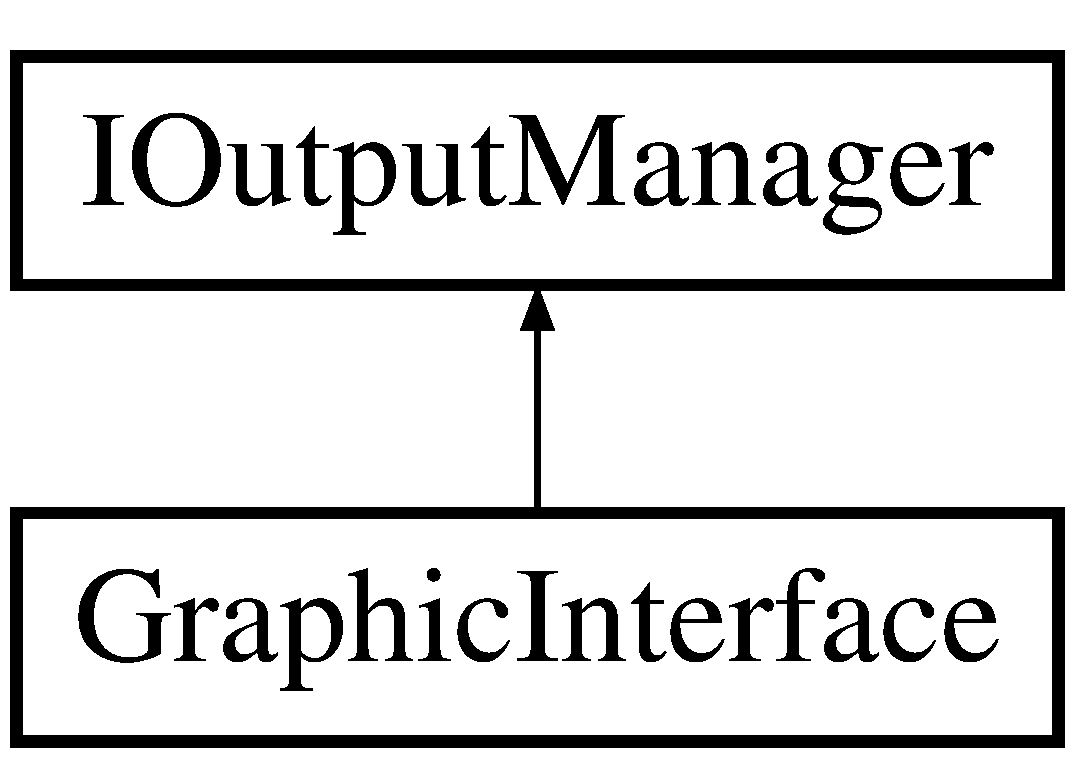
\includegraphics[height=2.000000cm]{class_i_output_manager}
\end{center}
\end{figure}
\subsection*{Public Member Functions}
\begin{DoxyCompactItemize}
\item 
virtual \mbox{\hyperlink{class_i_output_manager_a7442c5161bf453dc13605f7aaeeea2b5}{$\sim$\+I\+Output\+Manager}} ()=0
\begin{DoxyCompactList}\small\item\em virtual destructor to be implemented in the class implementing the interface \end{DoxyCompactList}\item 
\mbox{\Hypertarget{class_i_output_manager_a50a935d76cf10427b0977406a2338146}\label{class_i_output_manager_a50a935d76cf10427b0977406a2338146}} 
virtual void \mbox{\hyperlink{class_i_output_manager_a50a935d76cf10427b0977406a2338146}{load\+Level}} (\mbox{\hyperlink{class_output_data}{Output\+Data}})=0
\begin{DoxyCompactList}\small\item\em initialise S\+DL screen, read input data and create the maps and gamesprites in use \end{DoxyCompactList}\item 
\mbox{\Hypertarget{class_i_output_manager_aaebb6c7029ac00c7ce293272a5e854e3}\label{class_i_output_manager_aaebb6c7029ac00c7ce293272a5e854e3}} 
virtual void \mbox{\hyperlink{class_i_output_manager_aaebb6c7029ac00c7ce293272a5e854e3}{update}} (std\+::vector$<$ std\+::string $>$)=0
\begin{DoxyCompactList}\small\item\em update the screen based on the game state as determined by the logic manager \end{DoxyCompactList}\item 
\mbox{\Hypertarget{class_i_output_manager_aef1aaf499f3eee5927cb2833af39ce43}\label{class_i_output_manager_aef1aaf499f3eee5927cb2833af39ce43}} 
virtual void \mbox{\hyperlink{class_i_output_manager_aef1aaf499f3eee5927cb2833af39ce43}{update}} (User\+Input\+Type)=0
\begin{DoxyCompactList}\small\item\em for test purposes to bypass the logic component \end{DoxyCompactList}\item 
\mbox{\Hypertarget{class_i_output_manager_adc5ca9af7dc69324ee87233dcc7befc4}\label{class_i_output_manager_adc5ca9af7dc69324ee87233dcc7befc4}} 
virtual void {\bfseries show\+Game\+Over\+Screen} ()=0
\end{DoxyCompactItemize}


\subsection{Constructor \& Destructor Documentation}
\mbox{\Hypertarget{class_i_output_manager_a7442c5161bf453dc13605f7aaeeea2b5}\label{class_i_output_manager_a7442c5161bf453dc13605f7aaeeea2b5}} 
\index{I\+Output\+Manager@{I\+Output\+Manager}!````~I\+Output\+Manager@{$\sim$\+I\+Output\+Manager}}
\index{````~I\+Output\+Manager@{$\sim$\+I\+Output\+Manager}!I\+Output\+Manager@{I\+Output\+Manager}}
\subsubsection{\texorpdfstring{$\sim$\+I\+Output\+Manager()}{~IOutputManager()}}
{\footnotesize\ttfamily I\+Output\+Manager\+::$\sim$\+I\+Output\+Manager (\begin{DoxyParamCaption}{ }\end{DoxyParamCaption})\hspace{0.3cm}{\ttfamily [pure virtual]}, {\ttfamily [default]}}



virtual destructor to be implemented in the class implementing the interface 

Interface to be implemented by a class acting as the manager of the Output Component 

The documentation for this class was generated from the following files\+:\begin{DoxyCompactItemize}
\item 
C\+:/\+Users/\+User/source/repos/\+G\+A\+M\+E/\+G\+A\+M\+Esource/I\+Output\+Manager.\+h\item 
C\+:/\+Users/\+User/source/repos/\+G\+A\+M\+E/\+G\+A\+M\+Esource/I\+Output\+Manager.\+cpp\end{DoxyCompactItemize}

\hypertarget{class_i_storage_manager}{}\section{I\+Storage\+Manager Class Reference}
\label{class_i_storage_manager}\index{I\+Storage\+Manager@{I\+Storage\+Manager}}
Inheritance diagram for I\+Storage\+Manager\+:\begin{figure}[H]
\begin{center}
\leavevmode
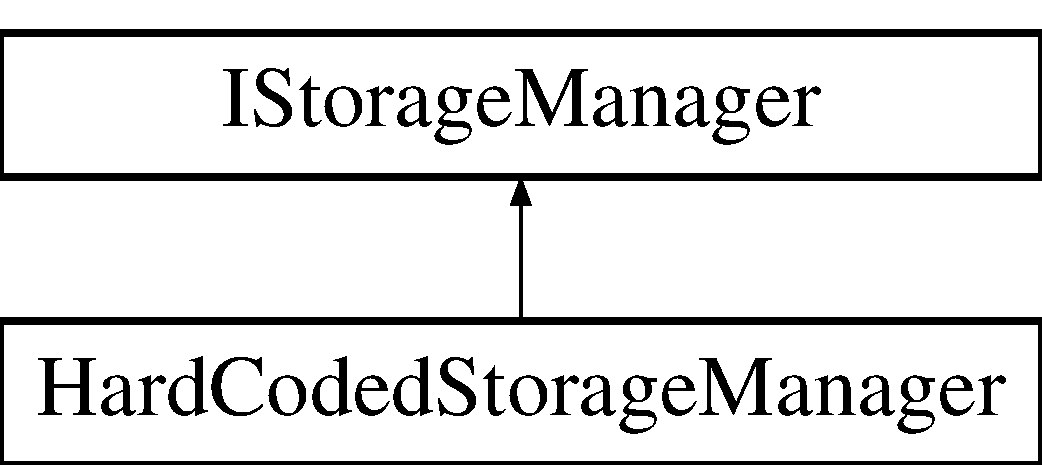
\includegraphics[height=2.000000cm]{class_i_storage_manager}
\end{center}
\end{figure}
\subsection*{Public Member Functions}
\begin{DoxyCompactItemize}
\item 
\mbox{\Hypertarget{class_i_storage_manager_a5e3d6fa4a26ce40e4a23a13138a2c055}\label{class_i_storage_manager_a5e3d6fa4a26ce40e4a23a13138a2c055}} 
virtual \mbox{\hyperlink{class_i_storage_manager_a5e3d6fa4a26ce40e4a23a13138a2c055}{$\sim$\+I\+Storage\+Manager}} ()=0
\begin{DoxyCompactList}\small\item\em virtual destructor to be implemented in the class implementing the interface \end{DoxyCompactList}\item 
\mbox{\Hypertarget{class_i_storage_manager_a8b8e56ec32e4780a5fda9fa26e18a70c}\label{class_i_storage_manager_a8b8e56ec32e4780a5fda9fa26e18a70c}} 
virtual \mbox{\hyperlink{class_storage_data}{Storage\+Data}} $\ast$ {\bfseries load\+Default\+Level} ()=0
\end{DoxyCompactItemize}


The documentation for this class was generated from the following files\+:\begin{DoxyCompactItemize}
\item 
C\+:/\+Users/\+User/source/repos/\+G\+A\+M\+E/\+G\+A\+M\+Esource/I\+Storage\+Manager.\+h\item 
C\+:/\+Users/\+User/source/repos/\+G\+A\+M\+E/\+G\+A\+M\+Esource/I\+Storage\+Manager.\+cpp\end{DoxyCompactItemize}

\hypertarget{class_keyboard_input_manager}{}\section{Keyboard\+Input\+Manager Class Reference}
\label{class_keyboard_input_manager}\index{Keyboard\+Input\+Manager@{Keyboard\+Input\+Manager}}
Inheritance diagram for Keyboard\+Input\+Manager\+:\begin{figure}[H]
\begin{center}
\leavevmode
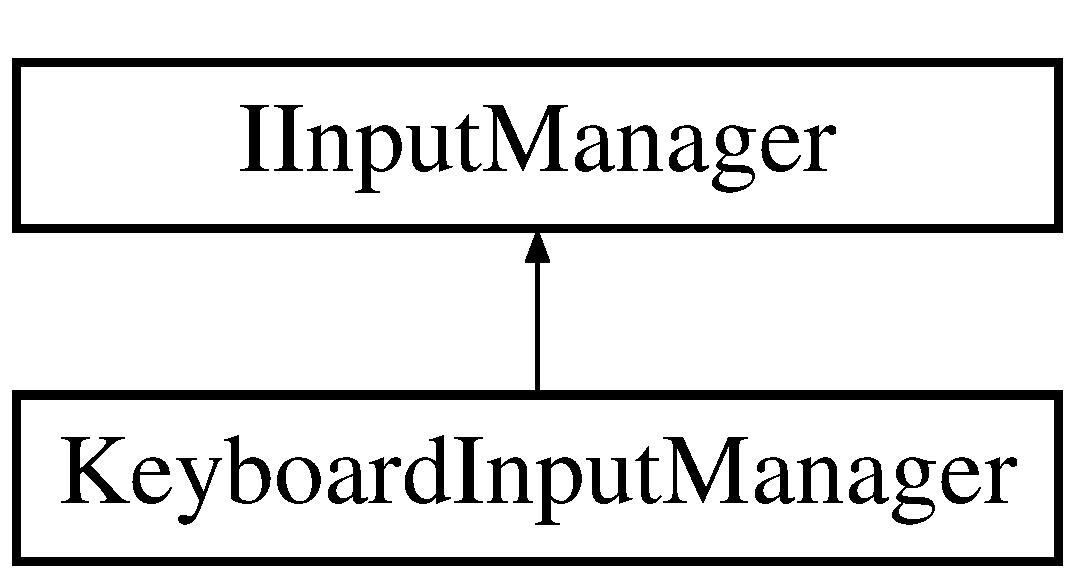
\includegraphics[height=2.000000cm]{class_keyboard_input_manager}
\end{center}
\end{figure}
\subsection*{Public Member Functions}
\begin{DoxyCompactItemize}
\item 
\mbox{\Hypertarget{class_keyboard_input_manager_a8cb1844b5ac0c023294a6a2378440c92}\label{class_keyboard_input_manager_a8cb1844b5ac0c023294a6a2378440c92}} 
User\+Input\+Type {\bfseries get\+Input} ()
\end{DoxyCompactItemize}


The documentation for this class was generated from the following files\+:\begin{DoxyCompactItemize}
\item 
C\+:/\+Users/\+User/source/repos/\+G\+A\+M\+E/\+G\+A\+M\+Esource/Keyboard\+Input\+Manager.\+h\item 
C\+:/\+Users/\+User/source/repos/\+G\+A\+M\+E/\+G\+A\+M\+Esource/Keyboard\+Input\+Manager.\+cpp\end{DoxyCompactItemize}

\hypertarget{class_logic_data}{}\section{Logic\+Data Class Reference}
\label{class_logic_data}\index{Logic\+Data@{Logic\+Data}}
\subsection*{Public Member Functions}
\begin{DoxyCompactItemize}
\item 
\mbox{\Hypertarget{class_logic_data_a182f7a8ffcbb3401e55e2922753c17bb}\label{class_logic_data_a182f7a8ffcbb3401e55e2922753c17bb}} 
{\bfseries Logic\+Data} (std\+::string s)
\end{DoxyCompactItemize}
\subsection*{Public Attributes}
\begin{DoxyCompactItemize}
\item 
\mbox{\Hypertarget{class_logic_data_a59c1bf0acf3ec2ea31d3bbf814740f2e}\label{class_logic_data_a59c1bf0acf3ec2ea31d3bbf814740f2e}} 
std\+::string {\bfseries data}
\end{DoxyCompactItemize}


The documentation for this class was generated from the following files\+:\begin{DoxyCompactItemize}
\item 
Logic\+Data.\+h\item 
Logic\+Data.\+cpp\end{DoxyCompactItemize}

\hypertarget{class_output_data}{}\section{Output\+Data Class Reference}
\label{class_output_data}\index{Output\+Data@{Output\+Data}}
\subsection*{Public Member Functions}
\begin{DoxyCompactItemize}
\item 
\mbox{\Hypertarget{class_output_data_a66eec456c0579b9945a412bb919f8f08}\label{class_output_data_a66eec456c0579b9945a412bb919f8f08}} 
\mbox{\hyperlink{class_output_data_a66eec456c0579b9945a412bb919f8f08}{Output\+Data}} (std\+::string)
\begin{DoxyCompactList}\small\item\em This is going to be a data package created by \mbox{\hyperlink{class_game_manager}{Game\+Manager}}, from Storage\+Data, for \mbox{\hyperlink{class_i_output_manager}{I\+Output\+Manager}}. \end{DoxyCompactList}\end{DoxyCompactItemize}
\subsection*{Public Attributes}
\begin{DoxyCompactItemize}
\item 
\mbox{\Hypertarget{class_output_data_aea2c1c5aff5523a159a410ff0e06b6fa}\label{class_output_data_aea2c1c5aff5523a159a410ff0e06b6fa}} 
std\+::string \mbox{\hyperlink{class_output_data_aea2c1c5aff5523a159a410ff0e06b6fa}{data}}
\begin{DoxyCompactList}\small\item\em string data given in a special format for loading each level \end{DoxyCompactList}\end{DoxyCompactItemize}


The documentation for this class was generated from the following files\+:\begin{DoxyCompactItemize}
\item 
G\+A\+M\+Esource/Output\+Data.\+h\item 
G\+A\+M\+Esource/Output\+Data.\+cpp\end{DoxyCompactItemize}

\hypertarget{class_player}{}\section{Player Class Reference}
\label{class_player}\index{Player@{Player}}
Inheritance diagram for Player\+:\begin{figure}[H]
\begin{center}
\leavevmode
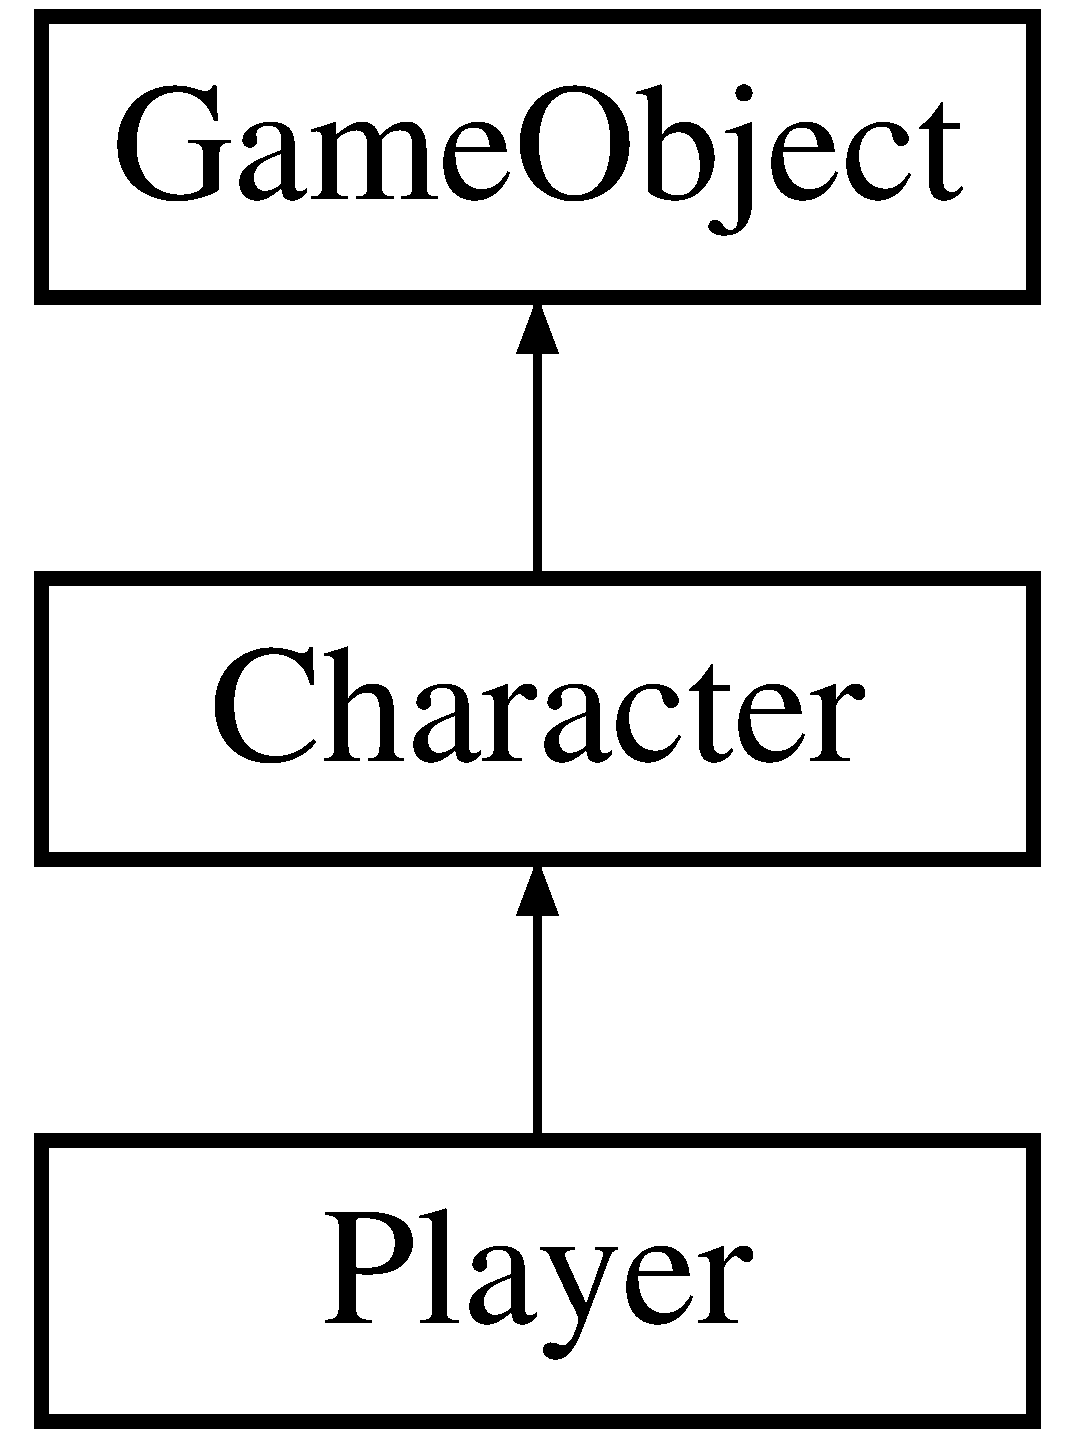
\includegraphics[height=3.000000cm]{class_player}
\end{center}
\end{figure}
\subsection*{Public Member Functions}
\begin{DoxyCompactItemize}
\item 
\mbox{\Hypertarget{class_player_abeb2eee0f7cf8bdd9ebbe6d1fb7d7641}\label{class_player_abeb2eee0f7cf8bdd9ebbe6d1fb7d7641}} 
{\bfseries Player} (std\+::string, int, int, int)
\end{DoxyCompactItemize}


The documentation for this class was generated from the following files\+:\begin{DoxyCompactItemize}
\item 
C\+:/\+Users/\+User/source/repos/\+G\+A\+M\+E/\+G\+A\+M\+Esource/Player.\+h\item 
C\+:/\+Users/\+User/source/repos/\+G\+A\+M\+E/\+G\+A\+M\+Esource/Player.\+cpp\end{DoxyCompactItemize}

\hypertarget{class_power_up}{}\section{Power\+Up Class Reference}
\label{class_power_up}\index{Power\+Up@{Power\+Up}}


A \mbox{\hyperlink{class_game_object}{Game\+Object}} that can be consumed by the player to change its attributes.  




{\ttfamily \#include $<$Power\+Up.\+h$>$}

Inheritance diagram for Power\+Up\+:\begin{figure}[H]
\begin{center}
\leavevmode
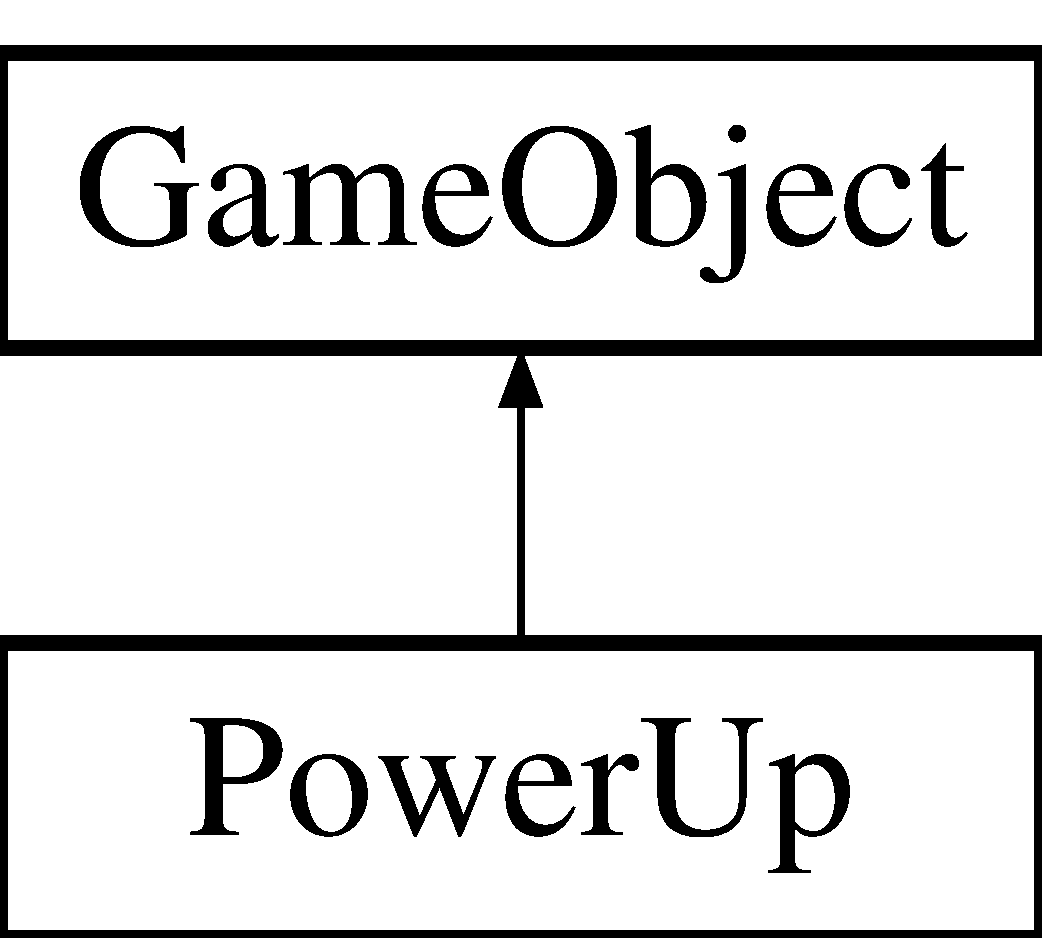
\includegraphics[height=2.000000cm]{class_power_up}
\end{center}
\end{figure}
\subsection*{Public Member Functions}
\begin{DoxyCompactItemize}
\item 
\mbox{\Hypertarget{class_power_up_a1146d214489e9f66e80b0d9905ce6aef}\label{class_power_up_a1146d214489e9f66e80b0d9905ce6aef}} 
{\bfseries Power\+Up} (const std\+::string, int, int, int)
\item 
\mbox{\Hypertarget{class_power_up_a0358e4edc1c61e26e0c7018b3ebef118}\label{class_power_up_a0358e4edc1c61e26e0c7018b3ebef118}} 
void \mbox{\hyperlink{class_power_up_a0358e4edc1c61e26e0c7018b3ebef118}{set\+Nr\+Of\+Lives}} (int)
\begin{DoxyCompactList}\small\item\em set the number of lives to be given \end{DoxyCompactList}\item 
\mbox{\Hypertarget{class_power_up_a20b1f2fa6a06891bdac68103f16816f1}\label{class_power_up_a20b1f2fa6a06891bdac68103f16816f1}} 
int \mbox{\hyperlink{class_power_up_a20b1f2fa6a06891bdac68103f16816f1}{get\+Nr\+Of\+Lives}} ()
\begin{DoxyCompactList}\small\item\em return number of lives that the power-\/up gives \end{DoxyCompactList}\end{DoxyCompactItemize}


\subsection{Detailed Description}
A \mbox{\hyperlink{class_game_object}{Game\+Object}} that can be consumed by the player to change its attributes. 

The documentation for this class was generated from the following files\+:\begin{DoxyCompactItemize}
\item 
G\+A\+M\+Esource/logic/Power\+Up.\+h\item 
G\+A\+M\+Esource/logic/Power\+Up.\+cpp\end{DoxyCompactItemize}

\hypertarget{class_random_input_generator}{}\section{Random\+Input\+Generator Class Reference}
\label{class_random_input_generator}\index{Random\+Input\+Generator@{Random\+Input\+Generator}}


Test class.  




{\ttfamily \#include $<$Random\+Input\+Generator.\+h$>$}

Inheritance diagram for Random\+Input\+Generator\+:\begin{figure}[H]
\begin{center}
\leavevmode
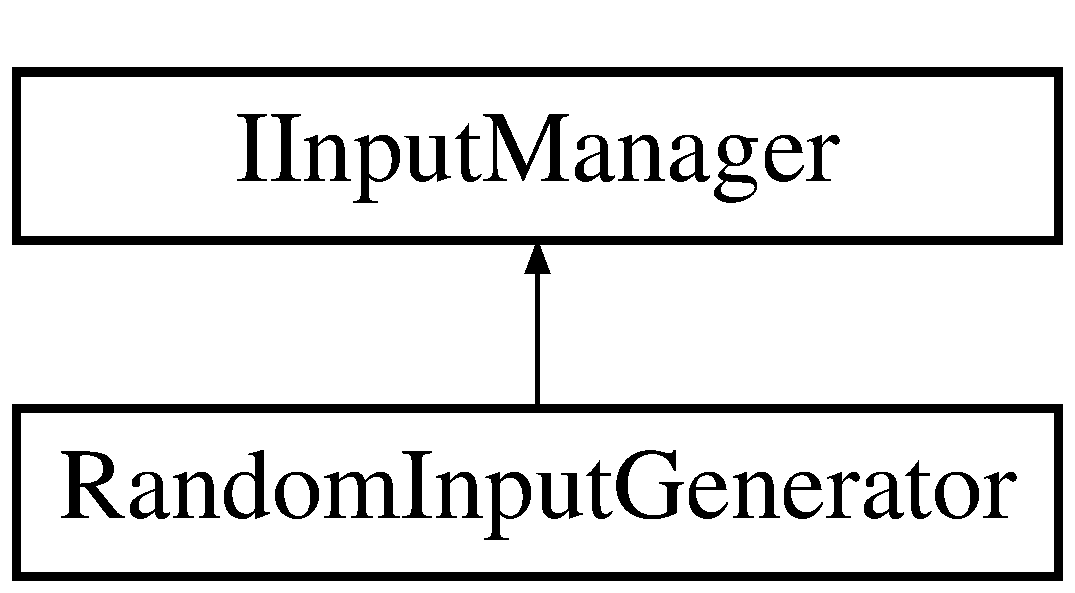
\includegraphics[height=2.000000cm]{class_random_input_generator}
\end{center}
\end{figure}
\subsection*{Public Member Functions}
\begin{DoxyCompactItemize}
\item 
\mbox{\Hypertarget{class_random_input_generator_a519c2556c497b6b5ab521334d39749d9}\label{class_random_input_generator_a519c2556c497b6b5ab521334d39749d9}} 
User\+Input\+Type \mbox{\hyperlink{class_random_input_generator_a519c2556c497b6b5ab521334d39749d9}{get\+Input}} ()
\begin{DoxyCompactList}\small\item\em Provides a single input from whichever source mapped as User\+Input\+Type. \end{DoxyCompactList}\end{DoxyCompactItemize}


\subsection{Detailed Description}
Test class. 

The documentation for this class was generated from the following files\+:\begin{DoxyCompactItemize}
\item 
G\+A\+M\+Esource/input/Random\+Input\+Generator.\+h\item 
G\+A\+M\+Esource/input/Random\+Input\+Generator.\+cpp\end{DoxyCompactItemize}

\hypertarget{class_storage_data}{}\section{Storage\+Data Class Reference}
\label{class_storage_data}\index{Storage\+Data@{Storage\+Data}}
\subsection*{Public Member Functions}
\begin{DoxyCompactItemize}
\item 
\mbox{\Hypertarget{class_storage_data_aef692cafa14b73abddaac22d527bd6de}\label{class_storage_data_aef692cafa14b73abddaac22d527bd6de}} 
{\bfseries Storage\+Data} (std\+::string ld, std\+::string od)
\end{DoxyCompactItemize}
\subsection*{Public Attributes}
\begin{DoxyCompactItemize}
\item 
\mbox{\Hypertarget{class_storage_data_adf525b90e94d0a64af74653b04ef9995}\label{class_storage_data_adf525b90e94d0a64af74653b04ef9995}} 
std\+::string {\bfseries logic\+Data}
\item 
\mbox{\Hypertarget{class_storage_data_adb52a97f028b7b65977a00df186f9cb8}\label{class_storage_data_adb52a97f028b7b65977a00df186f9cb8}} 
std\+::string {\bfseries output\+Data}
\end{DoxyCompactItemize}


The documentation for this class was generated from the following files\+:\begin{DoxyCompactItemize}
\item 
Storage\+Data.\+h\item 
Storage\+Data.\+cpp\end{DoxyCompactItemize}

%--- End generated contents ---

% Index
\backmatter
\newpage
\phantomsection
\clearemptydoublepage
\addcontentsline{toc}{chapter}{Index}
\printindex

\end{document}
